\documentclass[answers]{exam}
% 'texPreamble' contains formatting and macros. 
% https://github.com/pwesterbaan/scripts/tree/master/texmf/tex/latex/local
\usepackage{texPreamble}
\hypersetup{hidelinks}
\usepackage{relsize}
\usepackage{tkz-euclide}
\usepackage[titles]{tocloft}
\renewcommand{\cftsecleader}{\cftdotfill{\cftdotsep}}
\usetkzobj{all}
%% Externalize graphics and save in ./images/ folder
%% pdflatex -shell-escape <tex file>
%% The document can be compiled with the two following
%% lines commented out, but will recompile all figures
%% each time.
\usetikzlibrary{external}
\tikzexternalize[prefix=images/]
%% 
\usepackage{tabularx}
\extraheadheight{0.25in}
\extrafootheight{1.0in}
\extrawidth{1in}
% ----------------------------------------------------------------
\makeatletter
\title{Math 1080 Class notes\\[0.25\baselineskip]Fall 2020}
\author{\thefname\ \thelname}

\pagestyle{headandfoot}

%\firstpageheader{\@title\\\@date}{}{Math 1070}
%\firstpageheadrule

\newcommand*{\currentname}{\@currentlabelname}

\runningfootrule
\runningfooter{\parbox{0.45\linewidth}{\currentname}}{\thepage}{\@title}
\makeatother

\begin{document}
  %% Title
  \pagenumbering{roman}
  \vspace*{\stretch{1}}
  \begin{center}
    \makeatletter
    {\huge
    \@title}\\[\baselineskip]
    \@author\\[\baselineskip]
    Last updated:
    \@date\\
    \makeatother
  \end{center}
  \vspace*{\stretch{1}}
  \thispagestyle{empty}
  \pagebreak
  \pagestyle{headandfoot}

  \renewcommand{\contentsname}{Table Of Contents}
  \renewcommand\thesection{}
  \tableofcontents
  \newpage
  
  \makeatletter
  \firstpageheader{}{}{}
  \firstpagefooter{\parbox{0.45\linewidth}{\currentname}}{\thepage}{\@title}
  \firstpagefootrule
  \makeatother
  \pagenumbering{arabic}
  \setcounter{page}{1}
  %% everything else
  \relscale{1.4}

  \documentclass[mathNotesPreamble]{subfiles}
\begin{document}
%\relscale{1.4}
\section{5.5: Substitution Rule}
  \fbox{\parbox{0.9875\linewidth}{
    \textbf{Theorem 5.6: Substitution Rule for Indefinite Integrals}
  
    Let $u=g(x)$, where $g$ is differentiable on an interval, and let $f$ be continuous on the corresponding range of $g$. On that interval,
    \[\int f\parens{g(x)\vphantom{g(x)^1}}g'(x)\,dx=\int f(u)\,du\]
  }}
  \begin{ex*}
    We know
      \[\ddx\sbrkt{\frac{(2x+1)^4}{4}}=2(2x+1)^3\]
    Thus, if $f(x)=x^3$ and $g(x)=2x+1$ then $g'(x)=2$, so we let $u=2x+1$, then
    \begin{align*}
      \int 2(2x+1)^3\,dx&=\int f\parens{g(x)\vphantom{g(x)^1}}g'(x)\,dx\\
        &=\int u^3\,du\\
        &=\frac{u^4}{4}+C\\
        &=\frac{(2x+1)^4}{4}+C
    \end{align*}
  \end{ex*}
  \vspace*{\stretch{1}}
  
  \noindent
  \fbox{\parbox{0.9875\linewidth}{
    \textbf{Procedure: Substitution Rule (Change of Variables)}
    \begin{enumerate}
      \item Given an indefinite integral involving a composite function $f\parens{g(x)\vphantom{g(x)^1}}$, identify an inner function $u=g(x)$ such that a constant multiple of $g'(x)$ appears in the integrand.
      \item Substitute $u=g(x)$ and $du=g'(x)\,dx$ in the integral.
      \item Evaluate the new indefinite integral with respect to $u$.
      \item Write the result in terms of $x$ using $u=g(x)$.
    \end{enumerate}
  }}
  \pagebreak
  
  \begin{ex*}
    Evaluate the following integrals:
  \end{ex*}
  \begin{tasks}[after-item-skip=\stretch{1}](2)
    \task $\ds\int 2x(x^2+3)^4\,dx$
    \task $\ds\int (2x+1)^3\, dx$
    \task $\ds\int x^2\sqrt{x^3+1}\, dx$
    \task $\ds\int \theta\sqrt[4]{1-\theta^2}\,d\theta$
    \task $\ds\int\sqrt{4-t}\,dt$
    \task $\ds\int (2-x)^6\,dx$
  \end{tasks}
  \vspace*{\stretch{1}}
  \pagebreak
  
  \begin{ex*}
    Evaluate the following integrals:
  \end{ex*}
  \begin{tasks}[after-item-skip=\stretch{1}](2)
    \task $\ds\int\sec(2\theta)\tan(2\theta)\,d\theta$
    \task $\ds\int\csc^2\parens{\frac{t}{3}}\,dt$
    \task $\ds\int \frac{\sin(x)}{1+\cos^2(x)}\,dx$
    \task $\ds\int \frac{\tan\inv(x)}{1+x^2}\,dx$
  \end{tasks}
  \vspace*{\stretch{1}}
  
  \noindent
  The acceleration of a particle moving back and forth on a line is $a(t)=\frac{d^2s}{dt^2}=\pi^2\cos(\pi t)\ m/s^2$ for all $t$. If $s=0$ and $v=8\ m/s$ when $t=0$, find the value of $s$ when $t=1$ sec.
  \vspace*{\stretch{1}}
  \pagebreak
  
  \begin{ex*}
    Evaluate the following integrals:
  \end{ex*}
  \begin{tasks}[after-item-skip=\stretch{1}](2)
    \task $\ds\int(6x^2+2)\sin(x^3+x+1)\,dx$
    \task $\ds\int \frac{\sin(\theta)}{\cos^5(\theta)}\,d\theta$
    \task $\ds\int \frac{e^{\sqrt{x}}}{\sqrt x}\,dx$
    \task $\ds\int \frac{2^t}{2^t+3}\,dt$
  \end{tasks}
  \vspace*{\stretch{1}}
  \pagebreak
  
  \begin{tasks}[after-item-skip=\stretch{1}, resume](2)
    \task $\ds\int 6x^2 4^{x^3}\,dx$
    \task $\ds\int \frac{dx}{\sqrt{36-4x^2}}$
    \task $\ds\int \sin(t)\sec^2\parens{\cos(t)}\,dt$
    \task $\ds\int \frac{1}{\sqrt{x}\parens{1+\sqrt{x}}^2}\,dx$
  \end{tasks}
  \vspace*{\stretch{1}}
  \pagebreak

  \begin{tasks}[after-item-skip=\stretch{1}, resume](2)
    \task $\ds\int \frac{\sin(\sqrt{x})}{\sqrt x}\,dx$
    \task $\ds\int 5\cos(7x+5)\,dx$
    \task $\ds\int \frac{3}{\sqrt{1-25x^2}}\,dx$
    \task $\ds\int \frac{dx}{\sqrt{1-9x^2}}$
  \end{tasks}
  \vspace*{\stretch{1}}
  \pagebreak
  \begin{ex*}
    Evaluate the following integrals using the recommended substitution:
  \end{ex*}
  \begin{tasks}(2)
    \task $\ds\int \sec^2(x)\tan(x)\,dx$ \newline where $u=\tan(x)$.
    \task $\ds\int \sec^2(x)\tan(x)\,dx$ \newline where $u=\sec(x)$.
  \end{tasks}
  \vspace*{\stretch{1}}
  \begin{ex*}
  Solve the initial value problem: $\frac{dy}{dx}=4x(x^2+8)\inv[1/3], y(0)=0$.
  \end{ex*}
  \vspace*{\stretch{1}}
  \pagebreak
  \begin{ex*}
    Evaluate the following integrals:
  \end{ex*}
  \begin{tasks}[after-item-skip=\stretch{1}](2)
    \task $\ds\int xe\inv[x^2]\,dx$
    \task $\ds\int \frac{e^{1/x}}{x^2}\,dx$
    \task $\ds\int \frac{dt}{8-3t}$
    \task $\ds\int 5^t\sin(5^t)\,dt$
    \task $\ds\int \frac{e^w}{36+e^{2w}}\,dw$
  \end{tasks}
  \vspace*{\stretch{1}}
  \pagebreak

  \noindent
  \fbox{\parbox{0.9875\linewidth}{
    \textbf{Theorem 5.7: Substitution Rule for Definite Integrals}
  
    Let $u=g(x)$, where $g'$ is continuous on $\sbrkt{a,b}$, and let $f$ be continuous on the range of $g$. Then
      \[\int_a^b f\parens{g(x)\vphantom{g(x)^1}}g'(x)\,dx=\int_{g(a)}^{g(b)}f(u)\,du\]
  }}
  \begin{ex*}
    Evaluate the integrals:
  \end{ex*}
  \begin{tasks}[after-item-skip=\stretch{1}](2)
    \task $\ds\int_0^1 \frac{x^3}{\sqrt{x^4+9}}\,dx$
    \task $\ds\int_1^3 \frac{dt}{(t-4)^2}$
    \task $\ds\int_0^3 \frac{v^2+1}{\sqrt{v^3+3v+4}}\,dv$
    \task $\ds\int_0^1 2x\parens{4-x^2}\,dx$
  \end{tasks}
  \vspace*{\stretch{1}}
  \pagebreak
  
  \begin{tasks}[after-item-skip=\stretch{1}, resume](2)
    \task $\ds\int_2^3 \frac{x}{\sqrt[3]{x^2-1}}\,dx$
    \task $\ds\int_{0}^{\frac{\pi}{2}} \frac{\sin(x)}{1+\cos(x)}\,dx$
    \task $\ds\int_0^{\frac{\pi}{4}} \frac{\sin(x)}{\cos^2(x)}\,dx$
    \task $\ds\int_{-\frac{\pi}{12}}^{\frac{\pi}{8}} \sec^2(2y)\,dy$
  \end{tasks}
  \vspace*{\stretch{1}}
  \pagebreak
  
  \begin{tasks}[after-item-skip=\stretch{1}, resume](2)
    \task $\ds\int_0^1 (1-2x^9)\,dx$
    \task $\ds\int_0^1 (1-2x)^9\,dx$
    \task $\ds\int_0^{\frac{1}{2}} \frac{1}{1+4x^2}\,dx$
    \task $\ds\int_0^4 \frac{x}{x^2+1}\,dx$
  \end{tasks}
  \vspace*{\stretch{1}}
  \pagebreak
  
  \begin{tasks}[after-item-skip=\stretch{1}, resume](2)
    \task $\ds\int_0^\pi 3\cos^2(x)\sin(x)\,dx$
    \task $\ds\int_0^{\frac{\pi}{8}} \sec(2\theta)\tan(2\theta)\,d\theta$
    \task $\ds\int_0^1 (3t-1)^{50}\,dt$
    \task $\ds\int_0^3 \frac{1}{5x+1}\,dx$
  \end{tasks}
  \vspace*{\stretch{1}}
  \pagebreak
  
  \begin{tasks}[after-item-skip=\stretch{1}, resume](2)
    \task $\ds\int_0^1 xe\inv[x^2]\,dx$
    \task $\ds\int_e^{e^4} \frac{1}{x\sqrt{\ln(x)}}\,dx$
    \task $\ds\int_0^{\frac{1}{2}} \frac{\sin\inv(x)}{\sqrt{1-x^2}}\,dx$
    \task $\ds\int_0^1 \frac{e^z+1}{e^z+z}\,dz$
  \end{tasks}
  \vspace*{\stretch{1}}
  \pagebreak
  
  \begin{tasks}[after-item-skip=\stretch{1}, resume](2)
    \task $\ds\int_1^4 \frac{dy}{2\sqrt{y}\parens{1+\sqrt{y}}^2}$
    \task $\ds\int_{\ln\parens{\frac{\pi}{4}}}^{\ln\parens{\frac{\pi}{2}}} e^w\cos(e^w)\,dw$
    \task $\ds\int_0^{\frac{1}{8}} \frac{x}{\sqrt{1-16x^2}}\,dx$
    \task $\ds\int_1^{e^2} \frac{\ln(p)}{p}\,dp$
  \end{tasks}
  \vspace*{\stretch{1}}
  \pagebreak
  
  \begin{tasks}[after-item-skip=\stretch{1}, resume](2)
    \task $\ds\int_0^{\frac{\pi}{4}} e^{\sin^2(x)}\sin(2x)\,dx$
    \task $\ds\int_{-\pi}^{\pi} x^2\sin(7x^3)\,dx$
  \end{tasks}
  \vspace*{\stretch{1}}
  \begin{ex*}
    \textbf{Average velocity:} An object moves in one dimension with a velocity in $m/s$ given by $v(t)=8\sin(\pi t)+2t$. Find its average velocity over the time interval from $t=0$ to $t=10$, where $t$ is measured in seconds.
  \end{ex*}
  \vspace*{\stretch{1}}
  \pagebreak
  
  \begin{ex*}
    Prove $\ds\int \tan(x)\,dx=\ln\abs{\sec(x)}+C$.
  \end{ex*}
  \vspace*{\stretch{1}}
  \begin{ex*}
    Evaluate the integrals:
  \end{ex*}
  \begin{tasks}[after-item-skip=\stretch{1}](2)
    \task $\ds\int \frac{x}{(x-2)^3}\,dx$
    \task $\ds\int x\sqrt{x-1}\,dx$
  \end{tasks}
  \vspace*{\stretch{1}}
  \pagebreak
  
  \begin{tasks}[after-item-skip=\stretch{1}, resume](2)
    \task $\ds\int x^3(1+x^2)^\frac{3}{2}\,dx$
    \task $\ds\int \frac{y^2}{(y+1)^4}\,dy$
    \task $\ds\int (z+1)\sqrt{3z+2}\,dz$
    \task $\ds\int_0^1 \frac{x}{(x+2)^3}\,dx$
  \end{tasks}
  \vspace*{\stretch{1}}
  \pagebreak

  \begin{center}
    \fbox{\parbox{0.65\linewidth}{
      \textbf{Half-Angle Formulas}
      \begin{align*}
        \cos^2(\theta)&=\frac{1+\cos(2\theta)}{2}\\
        \sin^2(\theta)&=\frac{1-\cos(2\theta)}{2}
      \end{align*}
    }}
  \end{center}
  \begin{ex*}
    Evaluate the integrals:
  \end{ex*}
  \begin{tasks}[after-item-skip=\stretch{1}](2)
    \task $\ds\int \cos^2(x)\,dx$
    \task $\ds\int_{0}^{\frac{\pi}{2}}\cos^2(x)\,dx$
  \end{tasks}
  \vspace*{\stretch{1}}
  \pagebreak
  
  \begin{tasks}[after-item-skip=\stretch{1}, resume](2)
    \task $\ds\int \frac{1}{x^2}\cos^2\parens{\frac{1}{x}}\,dx$
    \task $\ds\int x\sin^2(x^2)\,dx$
    \task $\ds\int \sin^2\parens{\theta+\frac{\pi}{6}}\,d\theta$
    \task $\ds\int_{0}^{\frac{\pi}{4}} \cos^2(8\theta)\,d\theta$
  \end{tasks}
  \vspace*{\stretch{1}}
  \pagebreak
  
  \begin{ex*}
    If $f$ is continuous and $\ds\int_0^4 f(x)\,dx=10$, find $\ds\int_0^2 f(2x)\,dx$.
  \end{ex*}
  \vspace*{\stretch{1}}
  
  \begin{ex*}
    If $f$ is continuous and $\ds\int_0^9 f(x)\,dx=4$, find $\ds\int_0^3 xf(x^2)\,dx$.
  \end{ex*}
  \vspace*{\stretch{1}}
  
  \begin{ex*}
    Suppose $f$ is an even function with $\ds\int_0^8 f(x)\,dx=9$. Evaluate the following:
  \end{ex*}
  \begin{tasks}(2)
    \task $\ds\int_{-1}^1 x f(x^2)\,dx.$
    \task $\ds\int_{-2}^2 x^2 f(x^3)\,dx.$
  \end{tasks}
  \vspace*{\stretch{1}}
  \pagebreak
  
  \begin{ex*}
    Evaluate the integrals:
  \end{ex*}
  \begin{tasks}[after-item-skip=\stretch{1}](2)
    \task $\ds\int \sec^2(10x)\,dx$
    \task $\ds\int \tan^{10}(4x)\sec^2(4x)\,dx$
    \task $\ds\int\parens{x^\frac{3}{2}+8}^5\sqrt{x}\,dx$
    \task $\ds\int \frac{2x}{\sqrt{3x+2}}\,dx$
  \end{tasks}
  \vspace*{\stretch{1}}
  \pagebreak
  
  \begin{tasks}[after-item-skip=\stretch{1}, resume](2)
    \task $\ds\int \frac{7x^2+2x}{x}\,dx$
    \task $\ds\int \frac{e^x-e\inv[x]}{e^x+e\inv[x]}\,dx$
    \task $\ds\int_0^{\sqrt{3}} \frac{3}{9+x^2}\,dx$
    \task $\ds\int_0^{\frac{\pi}{6}} \frac{\sin(2y)}{\sin^2(y)+2}\,dy$
  \end{tasks}
  \vspace*{\stretch{1}}
  \pagebreak
  
  \begin{tasks}[after-item-skip=\stretch{1}, resume](2)
    \task $\ds\int \frac{\sec(z)\tan(z)}{\sqrt{\sec(z)}}\,dz$
    \task $\ds\int \frac{1}{\sin\inv(x)\sqrt{1-x^2}}\,dx$
    \task $\ds\int \frac{x}{\sqrt{4-9x^2}}\,dx$
    \task $\ds\int \frac{x}{1+x^4}\,dx$
  \end{tasks}
  \vspace*{\stretch{1}}
  \pagebreak
  
  \begin{tasks}[after-item-skip=\stretch{1}, resume](1)
    \task $\ds\int \frac{\cos\sqrt{\theta}}{\sqrt{\theta}\sin^2\sqrt{\theta}}\,d\theta$
    \task $\ds\int x^2\sqrt{2+x}\,dx$
    \task* $\ds\int \parens{\sin^5(x)+3\sin^3(x)-\sin(x)}\cos(x)\,dx$
  \end{tasks}
  \vspace*{\stretch{1}}
  \pagebreak
  
  \begin{tasks}[after-item-skip=\stretch{1}, resume](1)
    \task $\ds\int_{-\frac{\pi}{4}}^{\frac{\pi}{4}} \parens{x^3+x^4\tan(x)}\,dx$
    \task $\ds\int_{0}^{\frac{\pi}{2}} \cos(x)\sin\parens{\sin(x)}\,dx$
    \task $\ds\int \frac{1+x}{1+x^2}\,dx$
  \end{tasks}
  \vspace*{\stretch{1}}
  \pagebreak

  \noindent
  \begin{ex*}
    Evaluate these more challenging integrals:
  \end{ex*}
  \begin{tasks}[after-item-skip=\stretch{1}](1)
    \task $\ds\int \frac{dx}{\sqrt{1+\sqrt{1+x}}}$
  \end{tasks}
  \vspace*{\stretch{1}}
  \pagebreak  
  
  \begin{tasks}[after-item-skip=\stretch{1}, resume](1)
    \task $\ds\int x\sin^4(x^2)\cos(x^2)\,dx$
  \end{tasks}
  \vspace*{\stretch{1}}
  \pagebreak  
\end{document}

%  \documentclass[../mathNotesPreamble]{subfiles}
\begin{document}
%\relscale{1.4}
\section{6.1: Velocity and Net Change}

  \begin{defn*}[Position, Velocity, Displacement, and Distance]
    \begin{enumerate}
      \item 
        The \textbf{position} of an object moving along a line at time $t$, denoted $s(t)$, is the location of the object relative to the origin.
      \item 
        The \textbf{velocity} of an object at time $t$ is $v(t)=s'(t)$.
      \item 
        The \textbf{displacement} of the object between $t=a$ and $t=b>a$ is
          \[s(b)-s(a)=\int_a^b v(t)\,dt.\]
      \item 
        The \textbf{distance traveled} by the object between $t=a$ and $t=b>a$ is
          \[\int_a^b\abs{v(t)}\,dt\]
        where $\abs{v(t)}$ is the \textbf{speed} of the object at time $t$.
    \end{enumerate}
  \end{defn*}

  \vspace*{\stretch{1}}
  \begin{center}
    \includegraphics[width=0.325\linewidth, trim={0mm, 78.5mm, 0mm, 0mm}, clip]{../images/briggs_06_01/fig06_02}
    \hspace*{0.05\linewidth}
    \includegraphics[width=0.325\linewidth, trim={0mm, 0mm, 0mm, 95mm}, clip]{../images/briggs_06_01/fig06_02}
  \end{center}
  \vspace*{\stretch{1}}
  \pagebreak
  \begin{ex*}
    Suppose an object moves along a line with velocity (in ft/s) $v(t)=6-2t$, for $0\leq t\leq 5$, where $t$ is measured in seconds. 
  \end{ex*}
  \begin{itemize}[itemsep=\stretch{1}]
    \item 
      Find the displacement of the object on the interval $0\leq t\leq5$.
    \item 
      Find the distance traveled by the object on the interval $0\leq t\leq5$.
  \end{itemize}
  \vspace*{\stretch{1}}
  \begin{center}
    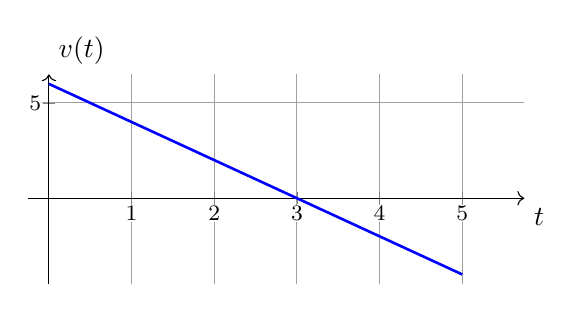
\begin{tikzpicture}
      \begin{axis}[
        grid=both, %major,minor
        grid style={line width=0.3pt, draw=gray!60},
        major grid style={line width=0.375pt, draw=gray!75},
        axis lines=center,
        axis line style={black,->},
        xmin=-0.25, xmax=5.75,
        ymin=-4.5, ymax=6.5,
        ticklabel style={font=\footnotesize,inner sep=0.5pt,fill=white,opacity=1.0, text opacity=1},
        xlabel=$t$, xlabel style={at={(ticklabel* cs:1)},anchor=north west},
        ylabel=$v(t)$, ylabel style={at={(ticklabel* cs:1)},anchor=south west},
        every axis plot/.append style={line width=0.95pt, color=blue, samples=100},
        width=0.65\linewidth, height=0.35\linewidth
        ]
         \addplot[-] expression[domain=0:5]{6-2*x};      
      \end{axis}
    \end{tikzpicture}
  \end{center}
  \pagebreak

  \begin{ex*}
    A cyclist rides down a long straight road at a velocity (in m/min) given by $v(t)= 400-20t$, for $0\leq t\leq 10$.
  \end{ex*}
  \begin{tasks}[after-item-skip=\stretch{1}, label=\textbullet](1)
    \task 
      How far does the cyclists travel in the first $5$ minutes?
    \task 
      How far does the cyclists travel in the first $10$ minutes?
    \task 
      How far has the cyclist traveled when her velocity is $250$ m/min?
  \end{tasks}
  \vspace*{\stretch{1}}
  \pagebreak

  \begin{ex*}
    The population of a community of foxes is observed to fluctuate on a 10-year cycle due to variations in the availability of prey.  When population measurements began ($t=0$), the population was $35$ foxes.  The growth rate in units of foxes/year was observed to be: 
  \end{ex*}
    \[P'(t)=5+10\sin\parens{\frac{\pi t}{5}}\]
  \begin{tasks}[after-item-skip=\stretch{1}, label=\textbullet](1)
    \task 
      Find $P(t)$.
    \task 
      Find the population of foxes after the first 5 years, rounded to the nearest whole number of foxes.
  \end{tasks}
  \vspace*{\stretch{1}}
  \pagebreak

  \vspace*{\stretch{0.75}}
  \begin{thmBox*}[Theorem 6.1: Position from Velocity]
    Given the velocity $v(t)$ of an object moving along a line and its initial position $s(0)$, the position function of the object for future times $t\geq 0$ is
      \[\underbrace{s(t)}_{\substack{\textnormal{position}\\ \textnormal{at $t$}}}=\underbrace{s(0)}_{\substack{\textnormal{initial}\\\textnormal{position}}}+\underbrace{\int_0^t v(x)\,dx}_{\substack{\textnormal{displacement}\\\textnormal{over $\sbrkt{0,t}$}}}.\]
  \end{thmBox*}
  \vspace*{\stretch{1}}

  \begin{thmBox*}[Theorem 6.2: Velocity from Acceleration]
    Given the acceleration $a(t)$ of an object moving along a line and its initial velocity $v(0)$, the velocity of the object for future times $t\geq 0$ is
      \[v(t)=v(0)+\int_0^t a(x)\,dx.\]
  \end{thmBox*}
  \vspace*{\stretch{1}}
  \pagebreak

  \begin{ex*}
    At $t=0$, a train approaching a station begins decelerating from a speed of $80$ miles/hour according to the acceleration function $a(t)=-1280(1+8t)^{-3}$, where $t\geq 0$ is measured in hours. The units of acceleration are mi/hr$^2$.
  \end{ex*}
  \begin{tasks}[after-item-skip=\stretch{1}, label=\textbullet](1)
    \task 
      Find the velocity of the train at $t=0.25$.
    \task 
      How far does the train travel in the first $15$ minutes ($1/4$ hour)? 
    \task 
      How long does it take the train to travel $9$ miles?
  \end{tasks}
  \vspace*{\stretch{1}}
  \pagebreak

  \vspace*{\stretch{1}}
  \begin{thmBox*}[Theorem 6.3: Net Change and Future Value]
    Suppose a quantity $Q$ changes over time at a known rate $Q'$. Then the \textbf{net change} in $Q$ between $t=a$ and $t=b>a$ is
      \[\underbrace{Q(b)-Q(a)}_{\textnormal{net change in }Q}=\int_a^b Q'(t)\,dt.\]
    Given the initial value $Q(0)$, the \textbf{future value} of $Q$ at time $t\geq 0$ is
      \[Q(t)=Q(0)+\int_0^t Q'(x)\,dx.\]
  \end{thmBox*}
  \vspace*{\stretch{1}}

  \begin{center}
    \scalebox{0.925}{
    \begin{tabular}{@{}l@{\hspace*{12.5mm}}l@{}}\toprule
      \textbf{Velocity-Displacement Problems}& \textbf{General Problems}\\[5pt]
      Position $s(t)$& Quantity $Q(t)$ (such as volume or population)\\[5pt]
      Velocity: $s'(t)=v(t)$& Rate of change: $Q'(t)$\\
      Displacement: $\ds s(b)-s(a)=\int_a^b v(t)\,dt$& Net change: $\ds Q(b)-Q(a)=\int_a^b Q'(t)\,dt$\\
      Future position: $\ds s(t)=s(0)+\int_0^t v(x)\,dx$& Future value of $Q$: $\ds Q(t)=Q(0)+\int_0^t Q'(x)\,dx$\\\bottomrule
    \end{tabular}}
  \end{center}
  \vspace*{\stretch{1}}
  \pagebreak

\end{document}

%  \documentclass[../mathNotesPreamble]{subfiles}
\begin{document}
\relscale{1.4}
  \section*{6.2: Regions Between Curves}

  \begin{defn*}[Area of a Region Between Two Curves]
    Suppose $f$ and $g$ are continuous functions with $f(x)\geq g(x)$ on the interval $\sbrkt{a,b}$. The area of the region bounded by the graphs of $f$ and $g$ on $\sbrkt{a,b}$ is
      \[A=\int_a^b \parens{f(x)-g(x)}\,dx.\]
  \end{defn*}

  \begin{defn*}[Area of a Region Between Two Curves with Respect to $y$]
    Suppose $f$ and $g$ are continuous functions with $f(y)\geq g(y)$ on the interval $\sbrkt{c,d}$. The area of the region bounded by the graphs $x=f(y)$ and $x=g(y)$ on $\sbrkt{c,d}$ is
      \[A=\int_c^d \parens{f(y)-g(y)}\,dy.\]
  \end{defn*}



\end{document}

%  \documentclass[../mathNotesPreamble]{subfiles}
\begin{document}
  \relscale{1.4}
  \section*{6.3: Volume by Slicing}

  \begin{thmBox*}[General Slicing Method]
    Suppose a solid object extends from $x=a$ to $y=b$, and the cross section of the solid perpendicular to the $x$-axis has an area given by a function $A$ that is integrable on $\sbrkt{a,b}$. The volume of the solid is
      \[V=\int_a^b A(x)\,dx.\]
  \end{thmBox*}

  \begin{thmBox*}[Disk Method about the $x$-Axis]
    Let $f$ be continuous with $f(x)\geq 0$ on the interval $\sbrkt{a,b}$. If the region $R$ bounded by the graph of $f$, the $x$-axis, and the lines $x=a$ and $x=b$ is revolved about the $x$-axis, the volume of the resulting solid of revolution is
      \[V=\int_a^b \pi\underbrace{f(x)^{\mathrlap{2}}}_{\substack{\textnormal{disk}\\\textnormal{radius}}}\,dx.\]
  \end{thmBox*}

  \begin{thmBox*}[Washer Method about the $x$-Axis]
    Let $f$ and $g$ be continuous functions with $f(x)\geq g(x)\geq 0$ on $\sbrkt{a,b}$. Let $R$ be the region bounded by $y=f(x)$, $y=g(x)$, and the lines $x=a$ and $x=b$. When $R$ is revolved about the $x$-axis, the volume of the resulting solid of revolution is
      \[V=\int_a^b \pi (\underbrace{f(x)^{\mathrlap{2}}}_{\substack{\textnormal{outer}\\\textnormal{radius}}}-\underbrace{g(x)^{\mathrlap{2}}}_{\substack{\textnormal{inner}\\\textnormal{radius}}}\phantom{^2})\,dx.\]
  \end{thmBox*}

  \begin{thmBox*}[Disk and Washer Methods about the $y$-Axis]
    Let $p$ and $q$ be continuous functions with $p(y)\geq q(y)\geq 0$ on $\sbrkt{c,d}$. Let $R$ be the region bounded by $x=p(y)$, $x=q(y)$, and the lines $y=c$ and $y=d$. When $R$ is revolved around the $y$-axis, the volume of the resulting solid of revolution is given by
      \[V=\int_c^d (\underbrace{p(y)^{\mathrlap{2}}}_{\substack{\textnormal{outer}\\\textnormal{radius}}}-\underbrace{q(y)^{\mathrlap{2}}}_{\substack{\textnormal{inner}\\\textnormal{radius}}}\phantom{^2})\,dy.\]
      If $q(y)=0$, the disk method results:
        \[V=\int_c^d \underbrace{p(y)^{\mathrlap{2}}}_{\substack{\textnormal{disk}\\\textnormal{radius}}}\,dy.\]
  \end{thmBox*} %TODO include figure 6.34

\end{document}

%  \documentclass[../mathNotesPreamble]{subfiles}
\begin{document}
%  \relscale{1.4}
  \section{6.4: Volume by Shells}

  \begin{thmBox*}[Volume by the Shell Method]
    Let $f$ and $g$ be continuous functions with $f(x)\geq g(x)$ on $\sbrkt{a,b}$. If $R$ is the region bounded by the curves $y=f(x)$ and $y=g(x)$ between the lines $x=a$ and $x=b$, the volume of the solid generated when $R$ is revolved about the $y$-axis is
      \[V=\int_a^b \underbrace{2\pi x\vphantom{)}}_{\substack{\textnormal{shell}\\\mathclap{\textnormal{circumference}}}} (\underbrace{f(x)-g(x)}_{\substack{\textnormal{shell}\\\textnormal{height}}})\,dx.\]
  \end{thmBox*}
  \begin{center}
    \includegraphics[width=0.6\linewidth]{../images/briggs_06_04/fig06_40}
    \vspace*{\stretch{1}}

    \includegraphics[width=0.5\linewidth]{../images/briggs_06_04/fig06_41}
  \end{center}
  \pagebreak

  \begin{ex*}
    Consider a general region $R$ revolved around the $y$-axis.
  \end{ex*}
  \begin{tasks}[after-item-skip=\stretch{1}, label=](1)
    \task 
      When using the \textbf{disk/washer} method, we integrate with respect to \underline{\hspace*{25mm}}
    \task 
      When using the \textbf{shell} method, we integrate with respect to \underline{\hspace*{25mm}}
  \end{tasks}
  \vspace*{\stretch{1}}
  \begin{ex*}
    Consider a general region $R$ revolved around the $x$-axis.
  \end{ex*}
  \begin{tasks}[after-item-skip=\stretch{1}, label=](1)
    \task 
      When using the \textbf{disk/washer} method, we integrate with respect to \underline{\hspace*{25mm}}
    \task 
      When using the \textbf{shell} method, we integrate with respect to \underline{\hspace*{25mm}}
  \end{tasks}
  \vspace*{\stretch{1}}
  \pagebreak

  \begin{ex*}
    Consider the region bounded between $y=x^3$, $y=8$ and $x=0$.
  \end{ex*}
  \begin{flushright}
    \begin{tikzpicture}
      \begin{axis}[
        grid style={line width=0.3pt, draw=gray!60},
        axis lines=center,
        axis line style={black,->},
        xmin=-2.5, xmax=2.5,
        ymin=-9, ymax=12,
        ymajorticks=false,
        ticklabel style={font=\footnotesize,inner sep=0.5pt,fill=white,opacity=0.5, text opacity=1},
        every axis plot/.append style={line width=0.95pt, color=blue, samples=100},
        width=0.45\linewidth, height=0.3\linewidth
        ]
        \addplot[->, name path=A, ClemsonPurple] expression[domain=-2:2.1]{x^3} node[black, pos=0.8, right, font=\normalsize] {$x^3$};
        \addplot[->, name path=B, ClemsonPurple] [domain=-2.5:2.5] {8} node[black, pos=0.25, above, font=\normalsize] {$y=8$};
        \addplot[fill=HowardsRock!55, opacity=0.75] fill between[of=A and B, soft clip={domain=0:2}];
      \end{axis}
    \end{tikzpicture}
  \end{flushright}
  \begin{tasks}[after-item-skip=\stretch{1}, label=](1)
    \task 
      Use the disk/washer method to setup the integral that represents the volume of the solid generated by rotating the region about the $x$-axis.
    \task 
      about the $y$-axis.
    \task 
      Use the disk/washer method to setup the integral that represents the volume of the solid generated by rotating the region about the line $x=-1$.
    \task 
      about the line $y=8$.
  \end{tasks}
  \vspace*{\stretch{1}}
  \pagebreak

\begin{ex*}
    Consider the region $R$ bounded by $y=4-x^2$, $y=2$, and $x=1$. Use the shell method to setup the integral that represents the volume of the solid generated by rotating the region $R$ about the indicated axis of rotation.
  \end{ex*}
  \newcommand{\parabolicFig}{
    \begin{flushright}
      \vspace*{-\baselineskip}
      \begin{tikzpicture}[scale=0.925]
        \begin{axis}[
          grid style={line width=0.3pt, draw=gray!60},
          axis lines=center,
          axis line style={black,->},
          xmin=-2.7, xmax=2.7,
          ymin=-1, ymax=4.5,
          ymajorticks=false,
          ticklabel style={font=\footnotesize,inner sep=0.5pt,fill=white,opacity=0.5, text opacity=1},
          every axis plot/.append style={line width=0.95pt, color=blue, samples=100},
          width=0.45\linewidth, height=0.3\linewidth
          ]
          \addplot[->, name path=A, ClemsonPurple] expression[domain=-2.5:2.5]{4-x^2} node[black, pos=0.71, right, font=\normalsize, xshift=-2pt] {$4-x^2$};
          \addplot[-, name path=B, ClemsonOrange] [domain=-2.5:2.5] {2} node[black, pos=0.4, above, font=\normalsize] {$y=2$};
          \addplot[fill=HowardsRock!55, opacity=0.75] fill between[of=A and B, soft clip={domain=1:1.414}];
          \draw[ClemsonOrange] (axis cs: 1,-2)--(axis cs: 1,5);
        \end{axis}
      \end{tikzpicture}
    \end{flushright}
    }
  
  \begin{tasks}[after-item-skip=\stretch{1}, label=](1)
    \task 
      about $x$-axis,
      \parabolicFig
    \task 
      about $y$-axis,
      \parabolicFig
    \task 
      about the line $x=-2$,
      \parabolicFig
    \task 
      about the line $y=2$.
      \parabolicFig
  \end{tasks}
  \pagebreak

  \begin{ex*}
    Consider the region bounded by $y=\dfrac{1}{x+1}$ and $y=1-\dfrac{x}{3}$. Use both the disk/washer method and shell method to find the volume of the solid generated when $R$ is rotated about the $x$-axis.
  \end{ex*}
  \vspace*{\stretch{1}}
  \pagebreak

  \begin{ex*}
    Determine if the following statements are true.
  \end{ex*}
  \begin{tasks}[after-item-skip=\stretch{1}, label=](1)
    \task 
      When using the shell method, the axis of the cylindrical shells is parallel to the axis of revolution.
    \task 
      If a region is revolved about the $y$-axis, then the shell method must be used.
    \task 
      If a region is revolved about the $x$-axis, it is possible to use the disk/washer method and integrate with respect to $x$.
  \end{tasks}
  \vspace*{\stretch{1}}
  \pagebreak

\end{document}

%  \documentclass[../mathNotesPreamble]{subfiles}
\begin{document}
%  \relscale{1.4}
  \section{6.5: Length of Curves}

  \begin{defn*}[Arc Length for $y=f(x)$]
    Let $f$ have a continuous first derivative on the interval $\sbrkt{a,b}$. The length of the curve from $\parens{a, f(a)}$ to $\parens{b, f(b)}$ is
      \[L=\int_a^b \sqrt{1+f'(x)^2}\,dx.\]
  \end{defn*}

  \vspace*{\stretch{1}}
  \begin{center}
    \includegraphics[width=0.6\linewidth]{../images/briggs_06_05/fig06_55}
  \end{center}
  \vspace*{\stretch{1}}
  
  \begin{defn*}[Arc Length for $x=g(y)$]
    Let $g$ have a continuous first derivative on the interval $\sbrkt{c,d}$. The length of the curve from $\parens{g(c),c}$ to $\parens{g(d),d}$ is
      \[L=\int_c^d \sqrt{1+g'(y)^2}\,dy.\]
  \end{defn*}
  \pagebreak

  \begin{ex*}
    Using a geometric argument, we can see that the length of $f(x)=-\dfrac{3}{4}x+\dfrac{7}{2}$ on the interval $\sbrkt{-6,2}$ is $L=10$. Compute this using the arc-length formula.
  \end{ex*}
  \begin{flushright}
    \begin{tikzpicture}
      \begin{axis}[
        grid = both,
        grid style={line width=0.3pt, draw=gray!60},
        axis lines=center,
        axis line style={black,->},
        xmin=-6.75, xmax=3.25,
        ymin=-0.5, ymax=9,
        ymajorticks=false,
        ticklabel style={font=\footnotesize,inner sep=0.5pt,fill=white,opacity=0.5, text opacity=1},
        every axis plot/.append style={line width=0.95pt, color=blue, samples=100},
        width=0.45\linewidth, height=0.3\linewidth
        ]
        \addplot[-, name path=A, ClemsonPurple] expression[domain=-6:2]{-0.75*x+3.5} node[above right, pos=0.3, black, inner sep=0.5pt, opacity=0.75, text opacity=1.0] {$f(x)$};
        \addplot[dashed] (-6,8)--(-6,2)--(2,2);
        \addplot[soldot] coordinates{(-6,8)} node[above right, pos=0.3, black, inner sep=0.5pt, opacity=0.75, text opacity=1.0, font=\normalsize] {$(-6,8)$};
        \addplot[soldot] coordinates{(2,2)} node[above right, pos=0.3, black, inner sep=0.5pt, opacity=0.75, text opacity=1.0, font=\normalsize] {$(2,2)$};
      \end{axis}
    \end{tikzpicture}
  \end{flushright}
  \vspace*{\stretch{1}}
  \pagebreak

  \begin{ex*}
    Find the arc length of the curve $y=\dfrac{1}{4}x^2-\dfrac{1}{2}\ln(x)$, for $1\leq x\leq 2$.
  \end{ex*}
  \vspace*{\stretch{1}}
  \pagebreak

  \begin{ex*}
    Find the arc length of the curve $y=\dfrac{1}{3}x^{\sfrac{3}{2}}$ on $\sbrkt{0,12}$.
  \end{ex*}
  \vspace*{\stretch{1}}
  \pagebreak

  \begin{ex*}
    Find a curve that passes through $\parens{1,2}$ on $\sbrkt{2,6}$ whose arc length is computed using 
      \[\displaystyle \int_2^6 \sqrt{1+16x^{-2}}\,dx.\]
  \end{ex*}
  \vspace*{\stretch{1}}
  
  \begin{ex*}
    Suppose $f$ has length $L$ on $\sbrkt{a,b}$. Evaluate
      \[\int_{\sfrac{a}{c}}^{\sfrac{b}{c}}\sqrt{1+f'(cx)^2}\,dx.\]
  \end{ex*}
  \vspace*{\stretch{1}}
  \pagebreak

\end{document}

%  \documentclass[../mathNotesPreamble]{subfiles}
\begin{document}
%  \relscale{1.4}
  \section{6.6: Surface Area}

  \begin{defn*}[Area of a Surface of Revolution]
    Let $f$ be a nonnegative function with a continuous first derivative on the interval $\sbrkt{a,b}$. The area of the surface generated when the graph of $f$ on the interval $\sbrkt{a,b}$ is revolved around the $x$-axis is
      \[S=\int_a^b 2\pi f(x)\sqrt{1+f'(x)^2}\,dx.\]
  \end{defn*}

  \begin{center}
    \includegraphics[width=0.5\linewidth]{../images/briggs_06_06/fig06_60}
  \end{center}

  \begin{ex*}
    Find the exact area of the surface obtained by rotating the curve $y=x^3$, $0\leq x\leq 2$ about the $x$-axis.
  \end{ex*}
  \vspace*{\stretch{1}}
  \pagebreak

  \begin{ex*}
    Find the exact area of the surface obtained by rotating the curve $y=\sqrt{8x-x^2}$, $1\leq x\leq 7$ about the $x$-axis.
  \end{ex*}
  \vspace*{\stretch{1}}
  \pagebreak

  \begin{ex*}
    Find the exact area of the surface obtained by rotating the curve $y=\dfrac{1}{2}\parens{e^{x}+e^{-x}}$, $-\ln(2)\leq x\leq \ln(2)$ about the $x$-axis.
  \end{ex*}
  \vspace*{\stretch{1}}
  \pagebreak

  

\end{document}

%  \documentclass[../mathNotesPreamble]{subfiles}
\begin{document}
  \relscale{1.4}
  \section{6.7: Physical Applications}

  \begin{defn*}[Mass of a One-Dimensional Object]
    Suppose a thin bar or wire is represented by the interval $a\leq x\leq b$ with a density function $\rho$ (with units of mass per length). The \textbf{mass} of the object is
      \[m=\int_a^b \rho(x)\,dx.\]
  \end{defn*}

  \begin{ex*}
    A thin bar, represented by the interval $0\leq x\leq 4$, has density in units of kg/m given by $\rho(x)=5e^{-2x}$. What is the mass of the bar?
  \end{ex*}
  \vspace*{\stretch{1}}
  \pagebreak

  \begin{defn*}[Work]
    The work done by a variable force $F$ moving an object along a line from $x=a$ to $x=b$ in the direction of the force is
      \[W=\int_a^b F(x)\,dx.\]
  \end{defn*}

  \begin{ex*}
    According to \textbf{Hooke's Law}, the force required to keep a spring in a compressed or stretched position $x$ units from the equilibrium position is $F(x)=kx$, where the positive spring constant $k$ measures the stiffness of the spring.
    \vspace*{\baselineskip}

    Suppose a force of $40 N$ is required to stretch a spring 0.1$m$ from its equilibrium position. Assuming the spring obeys Hooke's Law, how much work is required to stretch the spring 0.4$m$ beyond is equilibrium position? 
  \end{ex*}
  \vspace*{\stretch{1}}
  \pagebreak

  \begin{ex*}
    Imagine a chain of length $L$ meters with constant density $\rho$ kg/m is hanging vertically. Using $g$ to represent the force due to gravity, the work required to lift the chain is
      \[W=\int_0^L \rho g\parens{L-y}\,dy\]
    A $50$ meter long chain hangs vertically from a cylinder attached to a winch. Assume there is no friction in the system and the chain has a density of $3$\nobreakspace kg/m. How much work is required to wind the entire chain onto the cylinder if a $60$-kg load is attached to the end of the chain? Use $g$ for the acceleration due to gravity.
  \end{ex*}
  \vspace*{\stretch{1}}
  \pagebreak

  \begin{ex*}
    A $30$-meter long rope hangs freely from a ledge. The rope has a density of $5$\nobreakspace kg/m.  How much work is done if the top $1/3$ of the rope is pulled up to the ledge? Use $g$ for the acceleration due to gravity.
  \end{ex*}
  \vspace*{\stretch{1}}
  \pagebreak

  \begin{thmBox*}[Procedure: Solving Pumping Problems]
    \begin{enumerate}
      \item 
        Draw a $y$-axis in the vertical direction (parallel to gravity) and choose a convenient origin. Assume the interval $\sbrkt{a,b}$ corresponds to the vertical extent of the fluid.
      \item 
        For $a\leq y\leq b$, find the cross-sectional area $A(y)$ of the horizontal slices and the distance $D(y)$ the slices must be lifted.
      \item 
        The work required to lift the water is
          \[W=\int_a^b \rho gA(y)D(y)\,dy.\]
    \end{enumerate}
  \end{thmBox*}

  \begin{ex*}
    
  \end{ex*}
  \vspace*{\stretch{1}}
  \pagebreak

  \begin{thmBox*}[Procedure: Solving Force-on-Dam Problems]
    \begin{enumerate}
      \item 
        Draw a $y$-axis on the face of the dam in the vertical direction and choose a convenient origin (often taken to be the base of the dam).
      \item 
        Find the width function $w(y)$ for each value of $y$ on the face of the dam.
      \item 
        If the base of the dam is at $y=0$ and the top of the dam is at $y=a$, then the total force on the dam is
          \[F=\int_a^b \rho g\underbrace{(a-y)}_{\textnormal{depth}}\underbrace{w(y)}_{\textnormal{width}}\,dy.\]
    \end{enumerate}
  \end{thmBox*}

\end{document}

%  \documentclass[../mathNotesPreamble]{subfiles}
\begin{document}
%  \relscale{1.4}
  \section{8.1: Basic Approaches (to Integration)}
  \begin{ex*}
    Derive the integral formula $\displaystyle\int \sec(ax)\,dx=\frac{1}{a}\ln\abs{\sec(ax)+\tan(ax)}+C$.
  \end{ex*}
  \vspace*{\stretch{1}}

  \begin{ex*}
    Evaluate $\displaystyle \int \frac{dx}{e^{3x}+e^{-3x}}$.
  \end{ex*}
  \vspace*{\stretch{1}}
  \pagebreak

  \begin{ex*}
    Evaluate $\displaystyle \int \frac{\sin(x)+\cos^4(x)}{\csc(x)}\,dx$.
    \hspace*{\stretch{1}}
      \textit{Note}: 
      $\begin{cases}
        \cos^2(x)\hspace*{-10pt}&=\dfrac{1+\cos(2x)}{2}\\[5pt]
        \sin^2(x)\hspace*{-10pt}&=\dfrac{1-\cos(2x)}{2}
      \end{cases}$
  \end{ex*}
  \vspace*{\stretch{1}}

  \begin{ex*}
    Evaluate $\displaystyle \int \frac{2x^2+3x-4}{x-2}\,dx$.
  \end{ex*}
  \vspace*{\stretch{1}}
  \pagebreak

  \begin{ex*}
    Evaluate $\displaystyle \int \frac{dx}{\sqrt{7-6x-x^2}}$.
  \end{ex*}
  \vspace*{\stretch{1}}
  \pagebreak
\end{document}

%  \documentclass[../mathNotesPreamble]{subfiles}
\begin{document}
%  \relscale{1.4}
  \section{8.2: Integration by Parts}
  \begin{thmBox*}[Integraton by Parts]
    Suppose $u$ and $v$ are differentiable functions. Then
      \[\int u\,dv=uv-\int v\,du.\]
  \end{thmBox*}
  A good mnemonic is ILATE.
  \vspace*{\stretch{1}}
  \pagebreak

  \begin{ex*}
    Evaluate $\displaystyle\int xe^{-\frac{x}{2}}\,dx$.
  \end{ex*}
  \vspace*{\stretch{1}}
  \pagebreak

  \begin{ex*}
    Find the area of the region between the $x$-axis and $f(x)=\displaystyle\frac{\ln(x)}{x^2}$ on $\sbrkt{1,e}$.
  \end{ex*}
  \vspace*{\stretch{1}}
  \pagebreak

  \begin{ex*}
    Evaluate $\displaystyle\int x^2 \cos(2x)\,dx$.
  \end{ex*}
  \vspace*{\stretch{1}}
  \pagebreak

  \begin{ex*}
    Evaluate $\displaystyle\int e^{-x}\sin(3x)\,dx$.
  \end{ex*}
  \vspace*{\stretch{1}}
  \pagebreak

  \begin{ex*}
    Evaluate $\displaystyle\int e^{4x}\cos(3x)\,dx$.
  \end{ex*}
  \vspace*{\stretch{1}}
  \pagebreak

  \begin{ex*}
    Derive the integral formula 
      \[\int \ln(x)\,dx+x\ln(x)-x+C\]
  \end{ex*}
  \vspace*{\stretch{1}}

  \begin{ex*}
    Evaluate $\displaystyle\int10\cos(\sqrt{x})\,dx$
  \end{ex*}
  \vspace*{\stretch{1}}
  \pagebreak

  \begin{thmBox*}[Integration by Parts for Definite Integrals]
    Let $u$ and $v$ be differentiable. Then
      \[\left.\int_a^b u(x) v'(x)\,dx= u(x)v(x)\right|_a^b -\int_a^b v(x)u'(x)\,dx\]
  \end{thmBox*}
  \begin{ex*}
    Evaluate $\displaystyle \int_1^e \ln(2x)\,dx$.
  \end{ex*}
  \vspace*{\stretch{1}}
  \pagebreak
\end{document}

%  \documentclass[../mathNotesPreamble]{subfiles}
\begin{document}
%  \relscale{1.4}
  \section{8.3: Trigonometric Integrals}
  \textbf{Important trigonometric identities}
  \vspace*{\stretch{1}}
  \begin{center}
    \begin{tabularx}{0.9\linewidth}{@{}
      >{\hsize=0.9\hsize}X
      >{\hsize=1.1\hsize}X
      @{}}\toprule
      Pythagorean Identities&
      \vspace*{0.25\baselineskip}
      $\sin^2(\theta)+\cos^2(\theta)=1$\\[4\baselineskip]\midrule
      %
      Angle sum formulas& 
      \vspace*{0.25\baselineskip}
      $\begin{aligned}
        \sin(\alpha\pm\beta)&=\sin(\alpha)\cos(\beta)\pm\cos(\alpha)\sin(\beta)\\[0.25\baselineskip]
        \cos(\alpha\pm\beta)&=\cos(\alpha)\cos(\beta)\mp\sin(\alpha)\sin(\beta)\\[0.25\baselineskip]
      \end{aligned}$\\\midrule
      %
      Double angle formulas&
      \vspace*{0.25\baselineskip}
      $\begin{aligned}
        \sin(2\theta)&=2\sin(\theta)\cos(\theta)\\[0.25\baselineskip]
        \cos(2\theta)&=\cos^2(\theta)-\sin^2(\theta)\\[0.25\baselineskip]
      \end{aligned}$\\\midrule
      %
      Half angle formulas&
      \vspace*{0.25\baselineskip}
      $\begin{aligned}
        \sin^2(\theta)&=\dfrac{1-\cos(2\theta)}{2}\\[0.25\baselineskip]
        \cos^2(\theta)&=\dfrac{1-\cos(2\theta)}{2}\\[0.25\baselineskip]
      \end{aligned}$\\\bottomrule
    \end{tabularx}
  \end{center}
  \vspace*{\stretch{1}}
  \pagebreak

  \textbf{Derivation of angle sum formulas}

  \noindent
  \begin{minipage}{0.5\linewidth}
    \begin{align*}
      \sin(\alpha)&=\frac{\overline{DE}}{\overline{EF}}=\dfrac{\overline{DE}}{\sin(\beta)}
       &\Rightarrow \overline{DE}=\sin(\alpha)\sin(\beta)\\[\baselineskip]
      %
      \cos(\alpha)&=\frac{\overline{DF}}{\overline{EF}}=\dfrac{\overline{DF}}{\sin(\beta)}
       &\Rightarrow \overline{DF}=\cos(\alpha)\sin(\beta)\\[\baselineskip]
      %
      \sin(\alpha)&=\frac{\overline{CE}}{\overline{AE}}=\dfrac{\overline{CE}}{\cos(\beta)}
       &\Rightarrow \overline{CE}=\sin(\alpha)\cos(\beta)\\[\baselineskip]
      %
      \cos(\alpha)&=\frac{\overline{AC}}{\overline{AE}}=\dfrac{\overline{AC}}{\cos(\beta)}
       &\Rightarrow \overline{AC}=\cos(\alpha)\cos(\beta)\\[\baselineskip]
    \end{align*}
  \end{minipage}%
  \begin{minipage}{0.45\linewidth}
    \begin{flushright}
      \begin{tikzpicture}[declare function={c=4; s=3; h=sqrt(c^2+s^2); FE=2.25;}]
        \coordinate (A) at (0,0);
        \coordinate (C) at (c,0);
        \coordinate (E) at (c,s);
        \coordinate (F) at ($(E)+(-FE*s/h,FE*c/h)$);
        \coordinate (B) at ($(C)!(F)!(A)$);
        \coordinate (D) at ($(F)!(E)!(B)$);

        \draw[fill=ClemsonOrange!50, opacity=0.5] (A) -- (C) -- (E) -- cycle;
        \draw[fill=ClemsonPurple!50, opacity=0.5, text opacity=1.0] (A) -- node[pos=0.5, above left] {$1$} (F) -- (E);
        \draw (F) -- (B) (D) -- (E);

        \node[below left, inner sep=1pt] at (A) {$A$};
        \node[below, inner sep=2pt] at (B) {$B$};
        \node[below right, inner sep=1pt] at (C) {$C$};
        \node[left, inner sep=1.5pt] at (D) {$D$};
        \node[right, inner sep=2pt] at (E) {$E$};
        \node[above, inner sep=2pt] at (F) {$F$};

        \tkzLabelAngle[pos = 1.05](C,A,E){$\alpha$}
        \tkzLabelAngle[pos = 1.05](D,F,E){$\alpha$}
        \tkzLabelAngle[pos = 1.05](E,A,F){$\beta$}

        \draw[decorate, decoration={brace, amplitude=5pt}] ($(B)-(0,20pt)$)--($(A)-(0,20pt)$) node[pos=0.5, below, inner sep=7.5pt] {$\cos(\alpha+\beta)$};
        \draw[decorate, decoration={brace, amplitude=5pt}] ($(A)-(10pt,0)$)--($(A|-F)-(10pt,0)$) node[pos=0.5, above, inner sep=7.5pt, sloped] {$\sin(\alpha+\beta)$};
      \end{tikzpicture}
    \end{flushright}
  \end{minipage}%

  \textbf{Derivation of the double angle formulas}

  \begin{align*}
    \sin(2\theta)&=\sin(\theta+\theta)
      =\sin(\theta)\cos(\theta)+\cos(\theta)\sin(\theta)
      =2\sin(\theta)\cos(\theta)\\[0.5\baselineskip]
    \cos(2\theta)&=\cos(\theta+\theta)
      =\cos(\theta)\cos(\theta)-\sin(\theta)\sin(\theta)
      =\cos^2(\theta)-\sin^2(\theta)
  \end{align*}
  \vspace*{\stretch{1}}

  \textbf{Derivation of the half angle formulas}

  \noindent
  Start with the cosine double angle formula:
  \begin{align*}
    \cos(2\theta)&=\cos^2(\theta)-\sin^2(\theta)
      =\boxed{2\cos^2(\theta)-1}
      =\boxed{1-2\sin^2(\theta)}
  \end{align*}
  Solve for either $\sin^2(\theta)$ or $\cos^2(\theta)$:
  \begin{align*}
    \sin^2(\theta)&=\frac{1-\cos(2\theta)}{2}&
    \cos^2(\theta)&=\frac{1+\cos(2\theta)}{2}
  \end{align*}
  \vspace*{\stretch{1}}
  \pagebreak

  \begin{ex*}
    Evaluate the integral $\displaystyle \int \cos^5(x)\,dx$.
  \end{ex*}
  \vspace*{\stretch{1}}
  \pagebreak

  \begin{ex*}
    Evaluate the integral $\displaystyle \int\sin^3(x)\cos^{3/2}(x)\,dx$.
  \end{ex*}
  \vspace*{\stretch{1}}
  \pagebreak

  \begin{ex*}
    Evaluate the integral $\displaystyle \int 20\sin^2(x)\cos^2(x)\,dx$
  \end{ex*}
  \vspace*{\stretch{1}}
  \pagebreak

  \begin{ex*}
    Evaluate the integral $\displaystyle \int\sec^6(x)\tan^4(x)\,dx$.
  \end{ex*}
  \vspace*{\stretch{1}}
  \pagebreak

  \begin{ex*}
    Evaluate the integral $\displaystyle \int 35\tan^5(x)\sec^4(x)\,dx$.
  \end{ex*}
  \vspace*{\stretch{1}}
  \pagebreak

  \begin{ex*}
    Consider the region bounded by $y=\sec(x)$ and $y=\cos(x)$ for $0\leq x\leq \nicefrac{\pi}{3}$. Find the volume of the solid generated when rotating this region about the line $y=-1$.
  \end{ex*}
  \begin{flushright}
    \begin{tikzpicture}[declare function={
      PI=3.141592653589793;}]
      \begin{axis}[
        axis lines=center,
        axis line style={black,->},
        xmin=-0.95*PI, xmax=0.95*PI,
        vasymptote=PI/3,  
        ymin=-1.75, ymax=2.5,
        xtick={-3.141592653589793,
               -2.0943951023931953,
               -1.0471975511965976,
               0.0,
               1.0471975511965976,
               2.0943951023931953,
               3.141592653589793},
        xticklabels={$\displaystyle -\pi$,
                     $\displaystyle \nicefrac{-2\pi}{3}$,
                     $\displaystyle \nicefrac{\pi}{3}$,
                     $\displaystyle 0$,
                     $\displaystyle \nicefrac{\pi}{3}$,
                     $\displaystyle \nicefrac{2\pi}{3}$,
                     $\displaystyle \pi$},
        height=1.75in, width=0.9*0.5\linewidth,
        ticklabel style={font=\footnotesize,inner sep=0.5pt,fill=white,opacity=1.0, text opacity=1},
        xlabel=$x$, xlabel style={at={(ticklabel* cs:1)},anchor=north west},
        ylabel=$y$, ylabel style={at={(ticklabel* cs:1)},anchor=south west},
        every axis plot/.append style={line width=0.95pt, color=blue, samples=100}
        ]
        \addplot[-, red, name path =A] expression[domain=-PI:PI]{cos(deg(x))} node[black, above left, pos=0.35, font=\normalsize, inner sep=1pt] {$y=\cos(x)$};
        \foreach \n in {-1,0,1}{
          \addplot[-, name path = B] expression[domain=\n*PI-0.9*PI/2:\n*PI+0.9*PI/2, unbounded coords=jump]{sec(deg(x))};
          \addplot[fill=ClemsonPurple!55] fill between[of=A and B, soft clip={domain=0:PI/3}];
        }
      \end{axis}
    \end{tikzpicture}
  \end{flushright}
  \vspace*{\stretch{1}}
  \pagebreak

  \begin{ex*}
    Find the length of the curve $y=\ln\parens{2\sec(x)}$ on the interval $\sbrkt{0,\nicefrac{\pi}{6}}$.
  \end{ex*}
  \vspace*{\stretch{1}}
  \pagebreak

  \vspace*{\stretch{1}}
  \begin{center}
    \renewcommand{\arraystretch}{1.65}
    \relscale{0.9}
    \begin{tabularx}{\linewidth}{@{}
      >{\hsize=0.65\hsize}X
      >{\hsize=1.35\hsize}X
      @{}}\toprule
      $\displaystyle \int \sin^m(x)\cos^n(x)\,dx$& \textbf{Strategy}\\
      $m$ odd and positive, $n$ real& 
      Split off $\sin(x)$, rewrite the resulting even power of $\sin(x)$ in terms of $\cos(x)$, and then use $u=\cos(x)$.\\
      %
      $n$ odd and positive, $m$ real& 
      Split off $\cos(x)$, rewrite the resulting even power of $\cos(x)$ in terms of $\sin(x)$, and then use $u=\sin(x)$.\\
      %
      $m$ and $n$ both even, nonnegative integers&
      Use half-angle formulas to transform the integrand into a polynomial in $\cos(2x)$, and apply the preceding strategies once again to powers of $\cos(2x)$ greater than $1$.\\
      \midrule
      $\displaystyle \int \tan^m(x)\sec^n(x)\,dx$\\
      $n$ even and positive, $m$ real& 
      Split off $\sec^2(x)$, rewrite the remaining even power of $\sec(x)$ in terms of $\tan(x)$, and use $u=\tan(x)$.\\
      %
      $m$ odd and positive, $n$ real&
      Split off $\sec(x)\tan(x)$, rewrite the remaining even power of $\tan(x)$ in terms of $\sec(x)$, and use $u=\sec(x)$.\\
      %
      $n$ even and positive, $n$ odd and positive&
      Rewrite $\tan^m(x)$ in terms of $\sec(x)$\\\midrule
      %
      $\displaystyle \int \sec^n(x)\,dx$\\
      $n$ odd&
      Use integration by parts with $u=\sec^{n-2}(x)$ and \newline$dv=\sec^2(x)\,dx$\\
      %
      $m$ even&
      Split off $\sec^2(x)$, rewrite the remaining powers of $\sec(x)$ in terms of $\tan(x)$, and use $u=\tan(x)$.\\\midrule
      %
      $\displaystyle \int \tan^m(x)\,dx$&
      Split off $\tan^2(x)$ and rewrite in terms of $\sec(x)$. Expand into difference of integrals substituting $u=\tan(x)$. Repeat the process as needed for remaining powers of $\tan(x)$.\\
      \bottomrule
    \end{tabularx}
  \end{center}
  \vspace*{\stretch{1}}
  \pagebreak

\end{document}

%  \documentclass[../mathNotesPreamble]{subfiles}
\begin{document}
%  \relscale{1.4}
  \section{8.4: Trigonometric Substitutions}

  \begin{ex*}
    Verify the formula for the area of a circle with radius $a$ by finding the area under $f(x)=\sqrt{a^2-x^2}$.
  \end{ex*}
  \begin{flushright}
    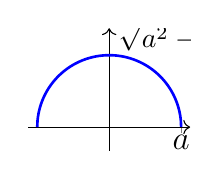
\begin{tikzpicture}
      \begin{axis}[
        axis lines=center,
        axis equal,
        axis line style={black,->},
        xmin=-4.5, xmax=4.5,
        ymin=-0.0625, ymax=4.25,
        xtick={4},
        xticklabels={$a$},
        ymajorticks=false,
        ticklabel style={font=\large,inner sep=0.5pt,fill=white,opacity=1.0, text opacity=1},
        every axis plot/.append style={line width=0.95pt, color=blue, samples=500}, 
        width=0.3\linewidth
        ]
        \addplot[-] expression[domain=-4:4]{sqrt(16-x^2)} node[pos=0.525, above right, black, font=\normalsize, inner sep=1pt] {$\sqrt{a^2-x^2}$};
      \end{axis}
    \end{tikzpicture}
  \end{flushright}
  \vspace*{\stretch{1}}

  \begin{center}
    \newcommand{\blankTriangle}[3]{
      \begin{tikzpicture}[scale=0.85]
        \coordinate (O) at (0,0);
        \coordinate (A) at (4,0);
        \coordinate (B) at (4,3);

        \tkzFillAngle[fill= ClemsonOrange!90,size=7.5mm, opacity=0.7](A,O,B);
        \tkzLabelAngle[pos = 1.1,font=\large](A,O,B){\color{black}$\theta$};
        \draw (O) -- node[below] {$#1$} (A) -- node[right] {$#2$} (B) -- node[above left] {$#3$} cycle;
      \end{tikzpicture}
    }
    \blankTriangle{\sqrt{a^2-u^2}}{u}{a} \hspace*{\stretch{1}}
    \blankTriangle{u}{a}{\sqrt{a^2-u^2}} \hspace*{\stretch{1}}
    \blankTriangle{a}{\sqrt{a^2-u^2}}{u}

    \addtolength{\jot}{15pt}
    \begin{alignat*}{4}\toprule
      &a^2-u^2 \hspace*{12mm}& 
      u&=a\sin(\theta),\hspace*{5mm}&
      &-\frac{\pi}{2}\leq \theta\leq \frac{\pi}{2}, \hspace*{2mm} \textnormal{ for } \abs{u}\leq a
       & \hspace*{12mm} a^2+a^2\sin^2(\theta)&=a^2\cos^2(\theta)\\
      %
      &a^2+u^2 &
      u&=a\tan(\theta),&
      &-\frac{\pi}{2}< \theta< \frac{\pi}{2},
       & a^2-a^2\tan^2(\theta)&=a^2\sec^2(\theta)\\
      %
      &u^2-a^2& 
      u&=a\sec(\theta),\ 
      &&\begin{cases}
        0\leq \theta< \frac{\pi}{2}, & \textnormal{ for } u\geq a\\
        \frac{\pi}{2}< \theta\leq \pi, & \textnormal{ for } u\leq -a
      \end{cases}
       & a^2\sec^2(\theta)-a^2&=a^2\tan^2(\theta)\\\bottomrule
    \end{alignat*}
  \end{center}
  \pagebreak

  \begin{ex*}
    $\displaystyle\int \frac{\sqrt{x^2-4}}{x^3}\,dx$
  \end{ex*}
  \vspace*{\stretch{1}}
  \pagebreak

  \begin{ex*}
    $\displaystyle\int \frac{\sqrt{16-x^2}}{x}\,dx$
  \end{ex*}
  \vspace*{\stretch{1}}
  \pagebreak

  \begin{ex*}
    $\displaystyle \int \frac{x^3}{\parens{25-4x^2}^{\nicefrac{3}{2}}}\,dx$
  \end{ex*}
  \vspace*{\stretch{1}}
  \pagebreak

  \begin{ex*}
    $\displaystyle \int_{0}^{\nicefrac{1}{3}} \frac{dx}{\parens{9x^2+1}^{\nicefrac{3}{2}}}$
  \end{ex*}
  \vspace*{\stretch{1}}
  \pagebreak

  \begin{ex*}
    $\displaystyle \int \frac{x}{\sqrt{x^2-2x+10}}$
  \end{ex*}
  \vspace*{\stretch{1}}
  \pagebreak

  \pagebreak

\end{document}

%  \documentclass[../mathNotesPreamble]{subfiles}
\begin{document}
%  \relscale{1.4}
  \section{8.5: Partial Fractions}
  \begin{ex*}
    Simplify $\displaystyle f(x)=\frac{1}{x-2}+\frac{2}{x+4}$ by finding a common denominator.
  \end{ex*}
  \vspace*{\stretch{0.5}}

  \begin{thmBox*}[Procedure: Partial Fractions with Simple Linear Factors]
    Suppose $f(x)=p(x)/q(x)$, where $p$ and $q$ are polynomials with no common factors and with the degree of $P$ less than the degree of $q$. Assume $q$ is the product of simple linear factors. The partial fraction decomposition is obtained as follows.
    \begin{enumerate}[label=\textbf{Step \arabic*:}, itemindent=1.5\labelwidth]
      \item \textbf{Factor the denominator $q$} in the form $(x-r_1)(x-r_2)\dots(x-r_n)$
      \item \textbf{Partial fraction decomposition}
        \[\frac{p(x)}{q(x)}=\frac{A_1}{(x-r_1)}+\frac{A_2}{(x-r_2)}+\dots+\frac{A_n}{(x-r_n)}.\]
      \item \textbf{Clear denominators} Multiply both sides of the equation in Step 2 by $q(x)=(x-r_1)(x-r_2)\dots(x-r_n)$
      \item \textbf{Solve for coefficients} Equate like powers of $x$ in Step 3 to solve for the undetermined coefficients $A_1,\dots,A_n$.
    \end{enumerate}
  \end{thmBox*}

  \begin{ex*}
    Perform partial fraction decomposition on $\displaystyle f(x)=\frac{3x}{x^2+2x-8}$.
  \end{ex*}
  \vspace*{\stretch{1}}
  \pagebreak

  \begin{ex*}
    $\displaystyle \int \frac{28x^3-56x^2+9}{x^2-2x}$
  \end{ex*}
  \vspace*{\stretch{1}}
  \pagebreak

  \begin{thmBox*}[Procedure: Partial Fractions for Repeated Linear Factors]
    Suppose the repeated linear factor $(x-r)^m$ appears in the denominator of a proper rational function in reduced form. The partial fraction decomposition has a partial fraction for each power of $(x-r)$ up to and including the $m$th power; that is, the partial fraction decomposition contains the sum  
    \[\frac{A_1}{(x-r)}+\frac{A_3}{(x-r)^2}+\frac{A_3}{(x-r)^3}+\dots+\frac{A_m}{(x-r)^m}\]
    where $A_1,\dots,A_m$ are constants to be determined.
  \end{thmBox*}
  \begin{ex*}
    Setup the partial fraction decomposition for $\displaystyle f(x)=\frac{x^3-8x+19}{x^4+3x^3}$.
  \end{ex*}
  \vspace*{\stretch{1}}
  \begin{ex*}
    Setup the partial fraction decomposition for $\displaystyle g(x)=\frac{2}{x^5-6x^4+9x^3}$.
  \end{ex*}
  \vspace*{\stretch{1}}
  \pagebreak

  \begin{ex*}
    Evaluate $\displaystyle \int \frac{x^2+1}{(2x-3)(x-2)^2}\,dx$.
  \end{ex*}
  \vspace*{\stretch{1}}
  \pagebreak

  \begin{ex*}
    Evaluate $\displaystyle \int \frac{8}{3x^3+7x^2+4x}\,dx$.
  \end{ex*}
  \vspace*{\stretch{1}}
  \pagebreak


  \begin{thmBox*}[Procedure: Partial Fractions with Simple Irreducible Quadratic Factors]
    Suppose a simple irreducible factor $ax^2+bx+c$ appears in the denominator of a proper rational function in reduced form. The partial fraction decomposition contains a term of the form
      \[\frac{Ax+B}{ax^2+bx+c},\]
    where $A$ and $B$ are unknown coefficients to be determined.
  \end{thmBox*}

  \begin{ex*}
    Perform partial fraction decomposition on the following fractions or identify them as irreducible.
  \end{ex*}
  \begin{tasks}[after-item-skip=\stretch{1}, label=, item-indent=0mm](1)
    \task $\displaystyle \frac{1}{x^2-13x+43}$
    \task $\displaystyle \frac{x^2}{(x-4)(x+5)}$
  \end{tasks}
  \vspace*{\stretch{1}}
  \pagebreak

  \begin{ex*}
    Perform partial fraction decomposition on the following fractions or identify them as irreducible.
  \end{ex*}
  \begin{tasks}[after-item-skip=\stretch{1}, label=, item-indent=0mm](1)
    \task $\displaystyle \frac{7}{(x^2+1)^2}$
    \task $\displaystyle \frac{1}{x^2+11x+28}$
  \end{tasks}
  \vspace*{\stretch{1}}
  \pagebreak

  \begin{ex*}
    Evaluate $\displaystyle \int \frac{4x}{(x+1)(x^2+1)}\,dx$
  \end{ex*}
  \vspace*{\stretch{1}}
  \pagebreak

  \begin{ex*}
    Evaluate $\displaystyle \int \frac{3x^2+2x+12}{(x^2+4)^2}\,dx$
  \end{ex*}
  \vspace*{\stretch{1}}
  \pagebreak

  \begin{ex*}
    Evaluate $\displaystyle \int \frac{1}{x\sqrt{1+2x}}\,dx$ using the substitution $u=\sqrt{1+2x}$.
  \end{ex*}
  \vspace*{\stretch{1}}
  \pagebreak

  \begin{thmBox*}[Summary: Partial Fraction Decomposition]
    Let $f(x)=p(x)/q(x)$ be a proper rational function in reduced form. Assume the denominator $q$ has been factored completely over the real numbers and $m$ is a positive integer.
    \begin{enumerate}
      \item \textbf{Simple linear factor:} A factor $x-r$ in the denominator requires the partial fraction $\dfrac{A}{x-r}$.
      \item \textbf{Repeated linear factor: } A factor $(x-r)^m$ with $m>1$ in the denominator requires the partial fractions
        \[\frac{A_1}{(x-r)}+\frac{A_2}{(x-r)^2}+\frac{A_3}{(x-r)^3}+\dots+\frac{A_m}{(x-r)^m}.\]
      \item \textbf{Simple irreducible quadratic factor: } An irreducible factor $ax^2+bx+c$ in the denominator requires the partial fraction 
        \[\frac{Ax+B}{ax^2+bx+c}.\]
      \item \textbf{Repeated irreducible quadratic factor:} An irreducible factor $(ax^2+bx+c)^m$ with $m>1$ in the denominator requires the partial fractions
        \[\frac{A_1x+B_1}{ax^2+bx+c}+\frac{A_2x+B_2}{(ax^2+bx+c)^2}+\dots+\frac{A_mx+B_m}{(ax^2+bx+c)^m}.\]
    \end{enumerate}
  \end{thmBox*}
  \vspace*{\stretch{1}}
  \pagebreak

\end{document}

%  \documentclass[../mathNotesPreamble]{subfiles}
\begin{document}
%  \relscale{1.4}
  \section{8.6: Integration Strategies}
    \begin{ex*}
      What integration methods can be used to evaluate the functions below?\newline (No need to evaluate the integral)
    \end{ex*}
    \begin{tasks}[after-item-skip=\stretch{1}, label=, item-indent=0pt](2)
      \task $\displaystyle \int \frac{1}{1-x^2}\,dx$
      \task $\displaystyle \int x\sec^2(x)\,dx$
      \task $\displaystyle \int \frac{x}{\sqrt{64-x^2}}\,dx$
      \task $\displaystyle \int \frac{x^3}{\sqrt{64-x^2}}\,dx$
    \end{tasks}
    \vspace*{\stretch{1}}
    \pagebreak

    \begin{ex*}
      Identify two integration techniques which can be used to evaluate 
        \[\displaystyle \int \frac{4-3x^2}{x(x^2-4)}\,dx.\]
    \end{ex*}
    \vspace*{\stretch{1}}

    \begin{ex*}
      Perform a substitution of variables to rewrite $\displaystyle \int x\sin(\sqrt{x})\,dx$.
    \end{ex*}
    \vspace*{\stretch{1}}
    \pagebreak

    \begin{ex*}
      $\displaystyle \int_{1}^{3} \frac{\tan\inv\parens{\sqrt{x}}}{x^{1/2}+x^{3/2}}\,dx$
    \end{ex*}
    \vspace*{\stretch{1}}
    \pagebreak

\end{document}

%  \documentclass[../mathNotesPreamble]{subfiles}
\begin{document}
%  \relscale{1.4}
  \section{8.9: Improper Integrals}
    \begin{defn*}[Improper Integrals over Infinite Intervals]
      \begin{enumerate}
        \item \label{infInterval_case1} If $f$ is continuous on $[a,\infty)$, then
          \[\int_a^\infty f(x)\,dx=\lim_{b\to \infty} \int_a^b f(x)\,dx.\]
        \item \label{infInterval_case2} If $f$ is continuous on $(-\infty,b]$, then
          \[\int_{-\infty}^b f(x)\,dx=\lim_{a\to -\infty} \int_a^b f(x)\,dx.\]
        \item \label{infInterval_case3} If $f$ is continuous on $(-\infty,\infty)$, then
          \[\int_{-\infty}^\infty f(x)\,dx=\lim_{a\to-\infty}\int_a^c f(x)\,dx+\lim_{b\to\infty}\int_c^b f(x)\,dx.\]
          where $c$ is any real number. It can be shown that the choice of $c$ does not affect the value or convergence of the original integral.
      \end{enumerate}
      If the limits in cases \ref{infInterval_case1}-- \ref{infInterval_case3} exist, then the improper integrals \textbf{converge}; otherwise they \textbf{diverge}.
    \end{defn*}

    \begin{ex*}
      Evaluate $\displaystyle \int_1^\infty \frac{\ln(x)}{x}\,dx$ and determine if the integral converges or diverges.
    \end{ex*}
    \vspace*{\stretch{1}}
    \pagebreak

    \begin{ex*}
      Evaluate $\displaystyle \int_{-\infty}^{\infty} \frac{e^{3x}}{1+e^{6x}}\,dx$.
    \end{ex*}
    \vspace*{\stretch{1}}
    \pagebreak

    \begin{ex*}
      For what values of $p$ does $\displaystyle \int_1^\infty \frac{1}{x^p}\,dx$ converge?
    \end{ex*}
    \vspace*{\stretch{1}}
    \pagebreak

    \begin{defn*}[Improper Integrals with Unbounded Integrand]
      \begin{enumerate}
        \item \label{unboundedIntegrand_case1} Suppose $f$ is continuous on $(a,b]$ with $\displaystyle \lim_{x\to a^+} f(x)=\pm\infty$. Then
          \[\int_a^b f(x)\,dx=\lim_{c\to a^+} \int_c^b f(x)\,dx.\]
        \item \label{unboundedIntegrand_case2} Suppose $f$ is continuous on $[a,b)$ with $\displaystyle \lim_{x\to b^-} f(x)=\pm\infty$. Then
          \[\int_a^b f(x)\,dx=\lim_{c\to b^-} \int_a^c f(x)\,dx.\]
        \item \label{unboundedIntegrand_case3} Suppose $f$ is continuous on $[a,b]$ except at the interior point $p$ where $f$ is unbounded. Then
          \[\int_a^b f(x)\,dx=\lim_{c\to p^-} \int_a^c f(x)\,dx + \lim_{d\to p^+}\int_d^b f(x)\,dx.\]
      \end{enumerate}
      If the limits in cases \ref{unboundedIntegrand_case1}-- \ref{unboundedIntegrand_case3} exist, then the improper integrals \textbf{converge}; otherwise, they \textbf{diverge}.
    \end{defn*}
    \pagebreak

    \begin{ex*}
      Determine which of the following integrals are improper integrals
    \end{ex*}
    \begin{tasks}[after-item-skip=\stretch{1}, label=, item-indent=0pt](2)
      \task $\displaystyle \int_0^1 \sec(x)\,dx$
      \task $\displaystyle \int_{\pi/2}^{3\pi/4} \tan(x)\,dx$
      \task $\displaystyle \int_1^e \ln(x)\,dx$
      \task $\displaystyle \int_0^1 \arctan(x)\,dx$
      \task $\displaystyle \int_0^{0.5} \ln(x)\,dx$
      \task $\displaystyle \int_{-10}^{-1} \frac{1}{x^{1/3}}\,dx$
    \end{tasks}
    \vspace*{\stretch{1}}
    \pagebreak

    \begin{ex*}
      Evaluate $\displaystyle \int_1^9 \frac{dx}{(x-1)^{2/3}}.$ Does this integral converge or diverge?
    \end{ex*}
    \vspace*{\stretch{1}}
    \pagebreak

    \begin{ex*}
      Evaluate $\displaystyle \int_{-1}^{1} \frac{e^{2/x}}{x^2}\,dx$. Does this integral converge or diverge?
    \end{ex*}
    \vspace*{\stretch{1}}
    \pagebreak

    \begin{thmBox*}[Theorem 8.2: Comparison Test for Improper Integrals]
      Suppose the functions $f$ and $g$ are continuous on the interval $[a,\infty)$, with\newline $f(x)\geq g(x)\geq 0$, for $x\geq a$.
      \begin{enumerate}
        \item If $\displaystyle \int_a^\infty f(x)\,dx$ converges, then $\displaystyle\int_a^\infty g(x)\,dx$ converges.
        \item If $\displaystyle \int_a^\infty g(x)\,dx$ diverges, then $\displaystyle\int_a^\infty f(x)\,dx$ diverges.
      \end{enumerate}
    \end{thmBox*}

    \begin{ex*}
      Determine if the integral $\displaystyle \int_2^\infty \frac{x^3}{x^4-x^3-1}\,dx$ converges or diverges.
    \end{ex*}
    \vspace*{\stretch{1}}
    \pagebreak

  \begin{ex*}[Gabriel's Horn]
      Let $R$ be the region bounded by the graph of $y=1/x$ and the $x$-axis for $x\geq 1$. 
    \end{ex*}
    \begin{tasks}[after-item-skip=\stretch{1}, label=, item-indent=0pt](1)
      \task What is the volume of the solid generated when $R$ is revolved around the $x$-axis?
      \task What is the surface area of the solid generated when $R$ is revolved about the $x$-axis?
    \end{tasks}
    \vspace*{\stretch{1}}
    \pagebreak

\end{document}

%  \documentclass[../mathNotesPreamble]{subfiles}
\begin{document}
%  \relscale{1.4}
  \section{10.1: An Overview of Sequences and Infinite Series}
    \begin{defn*}[Sequence]
      A \textbf{sequence} $\set{a_n}$ is an ordered list of numbers of the form
        \[\set{a_1,a_2,a_3,\dots,a_n,\dots}.\]
      A sequence may be generated by a \textbf{recurrence relation} of the form $a_\npo=f(a_n)$, for $n=1,2,3,\dots$, where $a_1$ is given. A sequence may also be defined with an \textbf{explicit formula} of the form $a_n=f(n)$, for $n=1,2,3,\dots$.
    \end{defn*}
    \begin{ex*}
      Consider the sequence $a_n=\frac{2^\npo}{2^n+1}$; Compute $a_1$, $a_2$, $a_3$, and $a_4$.
    \end{ex*}
    \vspace*{\stretch{1}}
    \pagebreak

    \begin{defn*}[Limit of a Sequence]
      If the terms of a sequence $\set{a_n}$ approach a unique number $L$ as $n$ increases--- that is, if $a_n$ can be made arbitrarily close to $L$ by taking $n$ sufficiently large--- then we say $\displaystyle\lim_{n\to \infty} a_n=L$ exists, and the sequence \textbf{converges} to $L$. If the terms of the sequence do not approach a single number as $n$ increases, the sequence has no limit, and the sequence \textbf{diverges}.
    \end{defn*}
    \begin{ex*}
      Determine if the sequence given by
        \[a_n=\frac{3+5n^2}{n+n^2}\]
      converges or diverges. If it converges, find the value that the sequence converges to.
    \end{ex*}
    \vspace*{\stretch{1}}

    \begin{ex*}
      Determine if the sequence given by
        \[a_n=(-1)^n\frac{3+5n^2}{n+n^2}\]
      converges or diverges. If it converges, find the value that the sequence converges to.
    \end{ex*}
    \vspace*{\stretch{1}}
    \pagebreak

    \begin{ex*}
      A ball is thrown upward to a height of 10 meters. After each bounce, the ball rebounds to $\sfrac{2}{3}$ of its previous height. Let $h_n$ be the height after the $n$th bounce. Find an explicit formula for the $n$th term of the sequence $\set{h_n}$.
    \end{ex*}
    \vspace*{\stretch{1}}
    \pagebreak

    \begin{defn*}[Infinite series]
      Given a sequence $\set{a_1, a_2, a_3,\dots}$, the sum of its terms
        \[a_1+a_2+a_3+\dots=\sum_{k=1}^\infty a_k\]
      is called an \textbf{infinite series}. The \textbf{sequence of partial sums} $\set{S_n}$ associated with this series has the terms
        \begin{align*}
          S_1&=a_1\\
          S_2&=a_1+a_2\\
          S_3&=a_1+a_2+a_3\\
          &\vdots\\
          S_n&=a_1+a_2+a_3+\dots+a_n=\sum_{k=1}^n a_k, &&\textnormal{ for } n=1,2,3,\dots.
        \end{align*}
      If the sequence of partial sums $\set{S_n}$ has a limit $L$, the infinite series \textbf{converges} to that limit, and we write
        \[\sum_{k=1}^\infty a_k=\lim_{n\to \infty}\underbrace{\sum_{k=1}^\infty a_k}_{S_n}=\lim_{n\to \infty}S_n=L.\]
      If the sequence of partial sums diverges, the infinite series also \textbf{diverges}.
    \end{defn*}
    \vspace*{\stretch{1}}
    \pagebreak

    \begin{ex*}
      Consider the infinite series $4+0.9+0.09+0.009+\dots$. Compute $S_1$, $S_2$, $S_3$, and $S_4$. What is the value of this series?
    \end{ex*}
    \vspace*{\stretch{1}}
    \pagebreak

    \begin{ex*}
      A sequence $\set{a_n}$ has partial sums given by the formula $S_n=5-\frac{1}{\sqrt{n}}$. 
    \end{ex*}
    \begin{tasks}[after-item-skip=\stretch{1}, label=, item-indent=0pt](1)
      \task What is the value of the series $\displaystyle\sum_{n=1}^\infty a_n$?
      \task What is the formula for $a_n$?
      \task What is the limit $\displaystyle\lim_{n\to \infty} a_n$?
    \end{tasks}
    \vspace*{\stretch{1}}
    \pagebreak

\end{document}

%  \documentclass[../mathNotesPreamble]{subfiles}
\begin{document}
%  \relscale{1.4}
  \section{10.2: Sequences}

  \begin{thmBox*}[Theorem 10.1: Limits of Sequences from Limits of Functions]
    Suppose $f$ is a function such that $f(n)=a_n$, for positive integers $n$. If \newline$\displaystyle \lim_{x\to \infty} f(x)=L$, then the limit of the sequence $\set{a_n}$ is also $L$, where $L$ may be $\pm\infty$.
  \end{thmBox*}

  \begin{ex*}
    Determine if the following sequences converge or diverge. If the sequence converges, find its limit.
  \end{ex*}
  \begin{tasks}[after-item-skip=\stretch{1}, label=, item-indent=0pt](2)
    \task $\set{e^{2n/(n+2)}}_{n=1}^{\infty}$
    \task $\set{\frac{(-1)^n}{n}}_{n=1}^{\infty}$
    \task $\set{\frac{\arctan(n)}{n}}_{n=1}^{\infty}$
    \task $\set{\frac{e^{-n}}{42\sin(e^{-n})}}_{n=1}^{\infty}$
  \end{tasks}
  \vspace*{\stretch{1}}
  \pagebreak

  \begin{thmBox*}[10.2: Limit Laws for Sequences]
    Assume the sequences $\set{a_n}$ and $\set{b_n}$ have limits $A$ and $B$, respectively. Then
      \begin{enumerate}
        \item $\displaystyle \lim_{n\to \infty}\parens{a_n\pm b_n}=A\pm B$
        \item $\displaystyle \lim_{n\to \infty} ca_n=cA$, where $c$ is a real number
        \item $\displaystyle \lim_{n\to \infty} a_nb_n=AB$
        \item $\displaystyle \lim_{n\to \infty} \frac{a_n}{b_n}= \frac{A}{B}$, provided $B\neq0$.
      \end{enumerate}
  \end{thmBox*}

  \begin{ex*}
    Consider the sequences $\set{a_n}$, $\set{b_n}$, $\set{c_n}$, and $\set{d_n}$ where
      \[a=\frac{1}{n},\quad b_n=n,\quad c_n=e^n,\quad \textnormal{ and } d_n=\sqrt{n}.\]
    Compute the following limits.
  \end{ex*}
  \begin{tasks}[after-item-skip=\stretch{1}, label=\Alph*., item-indent=17.5pt](4)
    \task $\displaystyle \lim_{n\to \infty} a_n$
    \task $\displaystyle \lim_{n\to \infty} b_n$
    \task $\displaystyle \lim_{n\to \infty} c_n$
    \task $\displaystyle \lim_{n\to \infty} d_n$
    \task $\displaystyle \lim_{n\to \infty} a_nb_n$
    \task $\displaystyle \lim_{n\to \infty} a_nc_n$
    \task $\displaystyle \lim_{n\to \infty} a_nd_n$
  \end{tasks}
  \vspace*{\stretch{1}}


  \noindent
  True or False: If for some sequence $\set{a_n}$ and $\set{b_n}$, $\displaystyle\lim_{n\to \infty}a_n=0$ and $\displaystyle\lim_{n\to \infty} b_n=\infty$, then $\displaystyle\lim_{n\to \infty} a_nb_n=0$.
  \pagebreak

  \begin{defn*}[Terminology for Sequences]
    \begin{enumerate}[label=\textbullet, itemsep=15pt]
      \item $\set{a_n}$ is \textbf{increasing} if $a_{n+1}>a_n$
      \item $\set{a_n}$ is \textbf{nondecreasing} if $a_{n+1}\geq a_n$
      \item $\set{a_n}$ is \textbf{decreasing} if $a_{n+1}< a_n$
      \item $\set{a_n}$ is \textbf{nonincreasing} if $a_{n+1}\leq a_n$
      \item $\set{a_n}$ is \textbf{monotonic} if it is either nonincreasing or nondecreasing (it moves in one direction)
      \item $\set{a_n}$ is \textbf{bounded above} if there is a number $M$ such that $a_n\leq M$, for all relevant values of $n$
      \item $\set{a_n}$ is \textbf{bounded below} if there is a number $N$ such that $a_n\geq N$, for all relevant values of $n$.
      \item If $\set{a_n}$ is bounded above and bounded below, then we say that $\set{a_n}$ is a \textbf{bounded} sequence.
    \end{enumerate}
  \end{defn*}
  \begin{ex*}
    Consider the sequence $\set{-n^2}_{n=1}^{\infty}$. What can we say about this sequence?
  \end{ex*}
  \vspace*{\stretch{1}}
  \pagebreak

  \begin{thmBox*}[Theorem 10.3: Geometric Sequences]
    Let $r$ be a real number. Then
      \[\lim_{n\to \infty} r^n =
        \begin{cases}
          0&\textnormal{ if } \abs{r}<1\\
          1&\textnormal{ if } r=1\\
          \textnormal{does not exist}& \textnormal{ if } r\leq -1 \textnormal{ or } r>1.
        \end{cases}
      \]
      If $r>0$, then $\set{r^n}$ is a monotonic sequence. If $r<0$, then $\set{r^n}$ oscillates.

      \begin{center}
        \begin{tikzpicture}[scale=2]
          \begin{axis}[
            axis line style={<->},
            xticklabel style = {yshift=-2pt},
            axis y line=none,
            axis x line*=center,
            ymin=0, ymax=1,
            xmin=-3, xmax=3,
            width=0.5\textwidth, height=24mm,
            xtick={-1,0,1},
            ticklabel style={font=\scriptsize,fill=white,opacity=1.0, text opacity=1},
            xlabel=$r$, xlabel style={at={(ticklabel* cs: 1.0), font=\normalsize}, below}
            ]
            \addplot[holdot, draw=black] coordinates{(-1,0)};
            \addplot[soldot, black] coordinates{(1,0)};
            \fill[ClemsonOrange, opacity=0.5] (-1,0) -- (1,0) -- (1,1) -- (-1,1) -- cycle;
            \fill[left color=white, right color=ClemsonPurple, opacity=0.25] (-2.75,0) -- (-1,0) -- (-1,1) -- (-2.75,1) -- cycle;
            \fill[right color=white, left color=ClemsonPurple, opacity=0.25] (2.75,0) -- (1,0) -- (1,1) -- (2.75,1) -- cycle;
            \draw[densely dashed, line width=0.75pt] (-1,0) -- (-1,1);
            \draw[line width=0.75pt] (1,0) -- (1,1);
            \node[font=\scriptsize, align=center] at (axis cs: -1.8,0.5) {Diverges\\ $r\leq -1$};
            \node[font=\scriptsize, align=center] at (axis cs: 0,0.5) {Converges\\ $-1<r\leq 1$};
            \node[font=\scriptsize, align=center] at (axis cs: 1.8,0.5) {Diverges\\ $r> 1$};
          \end{axis}
        \end{tikzpicture}
      \end{center}
    \vspace*{-\baselineskip}
  \end{thmBox*}

  \begin{ex*}
    Determine if the following sequences converge
  \end{ex*}
  \begin{tasks}[after-item-skip=\stretch{1}, label=, item-indent=0pt](2)
    \task $\displaystyle \set{\frac{3^{n+1}+3}{3^n}}$
    \task $\displaystyle \set{2^{n+1}3^{-n}}$
    \task $\displaystyle \set{\frac{(-1)^n}{2^n}}$
    \task $\displaystyle \set{\frac{75^{n-1}}{99^n}+\frac{5^n\sin(n)}{8^n}}$
  \end{tasks}
  \vspace*{\stretch{1}}
  \pagebreak

  \begin{thmBox*}[Theorem 10.4: Squeeze Theorem for Sequences]
    Let $\set{a_n}$, $\set{b_n}$, and $\set{c_n}$ be sequences with $a_n\leq b_n\leq c_n$, for all integers $n$ greater than some index $N$. If $\displaystyle\lim_{n\to \infty} a_n=\lim_{n\to \infty} c_n=L$, then $\displaystyle\lim_{n\to \infty} b_n=L$.
  \end{thmBox*}
  \begin{ex*}
    Find the limit of the sequence $b_n=\dfrac{9\cos(n)}{n^2+1}$.
  \end{ex*}
  \vspace*{\stretch{1}}

  \begin{thmBox*}[Theorem 10.5: Bounded Monotonic Sequence]
    A bounded monotonic sequence converges.
  \end{thmBox*}
  \pagebreak

  \begin{thmBox*}[Theorem 10.6: Growth Rates of Sequences]
    The following sequences are ordered according to increasing growth rates as $n\to\infty$; that is, if $\set{a_n}$ appears before $\set{b_n}$ in the list, then $\displaystyle\lim_{n\to \infty} \frac{a_n}{b_n}=0$ and $\displaystyle\lim_{n\to \infty} \frac{b_n}{a_n}=\infty$:
      \[\set{\parens{\ln n}^q} \hspace*{2.5pt} \ll \hspace*{2.5pt} \set{n^p} \hspace*{2.5pt} \ll \hspace*{2.5pt} \set{n^p\parens{\ln n}^r} \hspace*{2.5pt} \ll \hspace*{2.5pt} \set{n^{p+s}} \hspace*{2.5pt} \ll \hspace*{2.5pt} \set{b^n} \hspace*{2.5pt} \ll \hspace*{2.5pt} \set{n!} \hspace*{2.5pt} \ll \hspace*{2.5pt} \set{n^n}\]
  \end{thmBox*}

  \begin{ex*}
    Use growth rates to determine which of the following sequences converge.
  \end{ex*}
  \begin{tasks}[after-item-skip=\stretch{1}, label=,item-indent=0pt](1)
    \task $\displaystyle\set{\frac{\ln(n^{10})}{0.00001n}}$
    \task $\displaystyle\set{\frac{n^8\ln(n)}{n^{8.001}}}$
    \task $\displaystyle\set{\frac{n!}{10^n}}$
  \end{tasks}
  \vspace*{\stretch{1}}
  \pagebreak

  \begin{defn*}[Limit of a Sequence]
    The sequence $\set{a_n}$ converges to $L$ provided the terms of $a_n$ can be made arbitrarily close to $L$ by taking $n$ sufficiently large. More precisely, $\set{a_n}$ has the unique limit $L$ if, given any $\eps >0$, it is possible to find a positive integer $N$ (depending only on $\eps$) such that
      \[\abs{a_n-L}< \eps \qquad \textnormal{ whenever } n>N.\]
    If the \textbf{limit of a sequence} is $L$, we say the sequence \textbf{converges} to $L$, written
      \[\lim_{n\to \infty} a_n=L.\]
    A sequence that does not converge is said to \textbf{diverge}.
  \end{defn*}
  \vspace*{\stretch{1}}

\pagebreak
\end{document}

%  \documentclass[../mathNotesPreamble]{subfiles}
\begin{document}
%  \relscale{1.4}
  \section{10.3: Infinite Series}

  \noindent A \textbf{Geometric sum} with $n$ terms has the form
    \[S_n=a+ar+ar^2+\dots+ar^{n-1}=\sum_{k=0}^{n-1} ar^k\]

  \noindent\textbf{Derivation of partial sum formula:}
  \vspace*{\stretch{1}}

  \begin{thmBox*}[Theorem 10.7: Geometric Series]
    Let $a\neq 0$ and $r$ be real numbers. If $\abs{r}<1$, then $\displaystyle \sum_{k=0}^\infty ar^k=\frac{a}{1-r}$. If $\abs{r}\geq 1$, then the series diverges.

      \begin{center}
        \begin{tikzpicture}[scale=2]
          \begin{axis}[
            axis line style={<->},
            xticklabel style = {yshift=-2pt},
            axis y line=none,
            axis x line*=center,
            ymin=0, ymax=1,
            xmin=-3, xmax=3,
            width=0.5\textwidth, height=24mm,
            xtick={-1,0,1},
            ticklabel style={font=\scriptsize,fill=white,opacity=1.0, text opacity=1},
            xlabel=$r$, xlabel style={at={(ticklabel* cs: 1.0), font=\normalsize}, below}
            ]
            \addplot[holdot, draw=black] coordinates{(-1,0)(1,0)};
            \fill[ClemsonOrange, opacity=0.5] (-1,0) -- (1,0) -- (1,1) -- (-1,1) -- cycle;
            \fill[left color=white, right color=ClemsonPurple, opacity=0.25] (-2.75,0) -- (-1,0) -- (-1,1) -- (-2.75,1) -- cycle;
            \fill[right color=white, left color=ClemsonPurple, opacity=0.25] (2.75,0) -- (1,0) -- (1,1) -- (2.75,1) -- cycle;
            \draw[densely dashed, line width=0.75pt] (-1,0) -- (-1,1) (1,0) -- (1,1);
            \node[font=\scriptsize, align=center] at (axis cs: -1.8,0.5) {Diverges\\ $r\leq -1$};
            \node[font=\scriptsize, align=center] at (axis cs: 0,0.5) {Converges\\ $-1<r< 1$};
            \node[font=\scriptsize, align=center] at (axis cs: 1.8,0.5) {Diverges\\ $r\geq 1$};
          \end{axis}
        \end{tikzpicture}
      \end{center}
    \vspace*{-\baselineskip}
  \end{thmBox*}
  \pagebreak

  \begin{ex*}
    Evaluate the following geometric series or state that the series diverges
  \end{ex*}
  \begin{tasks}[after-item-skip=\stretch{1}, label=,item-indent=0pt](1)
    \task $\displaystyle\sum_{k=0}^\infty 1.1^k$
    \task $\displaystyle\sum_{k=0}^\infty e^{-k}$
    \task $\displaystyle\sum_{k=2}^\infty 3\parens{-0.75}^k$
    \task $\displaystyle\sum_{k=1}^\infty \frac{7}{10^k}$
  \end{tasks}
  \vspace*{\stretch{1}}
  \pagebreak

  \noindent \textbf{Telescoping Series:}

  \begin{ex*}
    Evaluate the following series
  \end{ex*}
  \begin{tasks}[after-item-skip=\stretch{1}, label=,item-indent=0pt](1)
    \task $\displaystyle\sum_{k=1}^\infty\ \cos\parens{\frac{1}{k^2}}-\cos\parens{\frac{1}{(k+1)^2}}$
    \task $\displaystyle\sum_{k=3}^\infty \frac{1}{(k-2)(k-1)}$
  \end{tasks}
  \vspace*{\stretch{1}}
  \pagebreak

  \begin{thmBox*}[Theorem 10.8: Properties of Convergent Series]
    \begin{enumerate}
      \item Suppose $\sum a_k$ converges to $A$ and $c$ is a real number. The series $\sum ca_k$ converges, and $\sum ca_k=c\sum a_k=cA$.
      \item Suppose $\sum a_k$ diverges. Then $\sum ca_k$ also diverges, for any real number $c\neq 0$.
      \item Suppose $\sum a_k$ converges to $A$ and $\sum b_k$ converges to $B$. The series $\sum \parens{a_k\pm b_k}$ converges and $\sum\parens{a_k\pm b_k}=\sum a_k \pm \sum b_k=A\pm B$.
      \item Suppose $\sum a_k$ diverges and $\sum b_k$ converges. Then $\sum \parens{a_k\pm b_k}$ diverges.
      \item If $M$ is a positive integer, then $\displaystyle \sum_{k=1}^\infty a_k$ and $\displaystyle\sum_{k=M}^\infty a_k$ either both converge or both diverge. In general, \textit{whether} a series converges does not depend on a finite number of terms added to or removed from the series. However, the \textit{value} of a convergent series does change if nonzero terms are added or removed.
    \end{enumerate}
  \end{thmBox*}

  \begin{ex*}
    Evaluate
  \end{ex*}
    $\displaystyle \sum_{k=1}^\infty \sbrkt{\frac{1}{2}\parens{\frac{2}{5}}^k+\frac{2}{3}\parens{\frac{1}{6}}^k}$
  \vspace*{\stretch{1}}
  \pagebreak

\end{document}

%  \documentclass[../mathNotesPreamble]{subfiles}
\begin{document}
%  \relscale{1.4}
  \section{10.4: The Divergence and Integral Tests}

  \begin{thmBox*}[Theorem 10.9: Divergence Test]
    If $\sum a_k$ converges, then $\displaystyle\lim_{k\to \infty} a_k=0$. Equivalently, if $\displaystyle\lim_{k\to \infty} a_k\neq 0$, then the series diverges.
  \end{thmBox*}
  \begin{ex*}
    If $\displaystyle\lim_{k\to \infty} a_k=1$, what can we conclude about $\displaystyle\sum_{k=1}^\infty a_k$?
  \end{ex*}
  \vspace*{\stretch{1}}
  \begin{ex*}
    If $\displaystyle\sum_{k=1}^\infty a_k=42$, what can we conclude about $\displaystyle\lim_{k\to \infty} a_k$?
  \end{ex*}
  \vspace*{\stretch{1}}
  \begin{ex*}
    If $\displaystyle \lim_{k\to \infty} a_k=0$, what can we conclude about $\displaystyle\sum_{k=1}^\infty a_k$?
  \end{ex*}
  \vspace*{\stretch{1}}
  \pagebreak

  \begin{ex*}
    Determine which of the following series diverge by the divergence test.
  \end{ex*}
  \begin{tasks}[after-item-skip=\stretch{1}, label=,item-indent=0pt](1)
    \task $\displaystyle\sum_{k=1}^\infty \frac{1}{\sqrt{k+1}}$
    \task $\displaystyle\sum_{k=1}^\infty \frac{k^3+100}{3k^3+k+1}$
    \task $\displaystyle\sum_{k=1}^\infty \frac{e^k}{k^2}$
  \end{tasks}
  \vspace*{\stretch{1}}
  \pagebreak

  \vspace*{\stretch{1}}
  \begin{center}
    \includegraphics[width=0.8\linewidth]{../images/briggs_10_04/PossibleImpossibleSeriesTable}
  \end{center}
  \vspace*{\stretch{1}}
  \begin{thmBox*}[Theorem 10.10: Harmonic Series]
    The harmonic series $\displaystyle\sum_{k=1}^\infty\frac{1}{k}=1+\frac{1}{2}+\frac{1}{3}+\frac{1}{4}+\frac{1}{5}+\dots$ diverges---even though the terms of the series approach zero.
  \end{thmBox*}
  \pagebreak

  \begin{thmBox*}[Theorem 10.11: Integral Test]
    Suppose $f$ is a continuous, positive, decreasing function, for $x\geq 1$, and let $a_k=f(k)$, for $k=1,2,3,\dots$. Then
      \[\sum_{k=1}^\infty a_k \textnormal{ and } \int_1^\infty f(x)\,dx\]
    either both converge or both diverge. In the case of convergence, the value of the integral is \textit{not} equal to the value of the series.
  \end{thmBox*}
  \begin{ex*}
    Which of the following series below satisfy all the conditions to use the Integral Test?
  \end{ex*}
  \begin{tasks}[after-item-skip=\stretch{1}, label=,item-indent=0pt](1)
    \task $\displaystyle\sum_{k=1}^\infty \arctan(k)$
    \task $\displaystyle\sum_{k=1}^\infty \frac{(-1)^k}{k^2}$
    \task $\displaystyle\sum_{k=1}^\infty \frac{1}{e^k}$
  \end{tasks}
  \vspace*{\stretch{1}}
  \pagebreak

  \begin{ex*}
    Consider the series
      \[\sum_{k=1}^\infty \frac{1}{k^p}\]
    Use the integral test to show that the Harmonic Series diverges. For what values of $p$ does this series converge?
  \end{ex*}
  \vspace*{\stretch{1}}
  \pagebreak

  \begin{thmBox*}[Theorem 10.12: Convergence of the $p$-series]
    The \textbf{$p$-series} $\displaystyle\sum_{k=1}^\infty \frac{1}{k^p}$ converges for $p>1$ and diverges for $p\leq 1$.
  \end{thmBox*}
  \begin{ex*}
    Determine if the following $p$-series converge or diverge.
  \end{ex*}
  \begin{tasks}[after-item-skip=\stretch{1}, label=,item-indent=0pt](2)
    \task $\displaystyle \sum_{k=1}^\infty \frac{1}{k^2}$
    \task $\displaystyle \sum_{k=1}^\infty k^{-1/3}$
    \task $\displaystyle \sum_{k=1}^\infty \frac{k^2}{k^\pi}$
    \task $\displaystyle \sum_{k=1}^\infty \frac{2}{k}$
    \task $\displaystyle \sum_{k=1}^\infty \frac{-3}{\sqrt[3]{k^4}}$
    \task $\displaystyle \sum_{k=1}^\infty \frac{k^3+1}{k^5}$
  \end{tasks}
  \vspace*{\stretch{1}}
  \pagebreak

  \begin{ex*}
    Apply the Integral Test to determine if the series $\displaystyle\sum_{k=1}^\infty \frac{1}{\sqrt{k+1}}$ converges or diverges.
  \end{ex*}
  \vspace*{\stretch{1}}
  \pagebreak

  \begin{thmBox*}[Theorem 10.13: Estimating Series with Positive Terms]
    Let $f$ be a continuous, positive, decreasing function, for $x\geq 1$, and let $a_k=f(k)$, for $k=1,2,3,\dots$. Let $S=\displaystyle\sum_{k=1}^\infty a_k$ be a convergent series and let $S_n=\displaystyle\sum_{k=1}^n a_k$ be the sum of the first $n$ terms of the series. The remainder $R_n=S-S_n$ satisfies 
      \[R_n < \int_n^\infty f(x)\,dx.\]
    Furthermore, the exact value of the series is bounded as follows:
      \[L_n=S_n+\int_{n+1}^\infty f(x)\,dx < \sum_{k=1}^\infty a_k < S_n+\int_n^\infty f(x)\,dx=U_n.\]
  \end{thmBox*}
  \begin{ex*}
    How many terms of the convergent $p$-series $\displaystyle\sum_{k=1}^\infty \frac{1}{k^2}$ must be summed to obtain an approximation that is within $10^{-3}$ of the exact value of the series?
  \end{ex*}
  \vspace*{\stretch{1}}

  \pagebreak
\end{document}

%  \documentclass[../mathNotesPreamble]{subfiles}
\begin{document}
%  \relscale{1.4}
  \section{10.5: Comparison Tests}

  \begin{thmBox*}[Theorem 10.14: Comparison Test]
    Let $\sum a_k$ and $\sum b_k$ be series with positive terms where $a_k\leq b_k$. 
    \begin{enumerate}
      \item If $\sum b_k$ converges, then $\sum a_k$ converges.
      \item If $\sum a_k$ diverges, then $\sum b_k$ diverges.
    \end{enumerate}
  \end{thmBox*}
  \begin{ex*}
    Use the comparison test to determine if the series $\displaystyle\sum_{k=1}^\infty \frac{k^2}{k^3-3}$ converges or diverges.
  \end{ex*}
  \vspace*{\stretch{1}}
  \pagebreak 

  \begin{thmBox*}[Theorem 10.15: Limit Comparison Test]
    Let $\sum a_k$ and $\sum b_k$ be series with positive terms and let
      \[\lim_{k\to \infty} \frac{a_k}{b_k}=L.\]
    \begin{enumerate}
      \item If $0<L<\infty$ (that is, $L$ is a finite positive number), then $\sum a_k$ and $\sum b_k$ either both converge or both diverge.
      \item If $L=0$ and $\sum b_k$ converges, then $\sum a_k$ converges.
      \item If $L=\infty$ and $\sum b_k$ diverges, then $\sum a_k$ diverges.
    \end{enumerate}
  \end{thmBox*}
  \begin{ex*}
    Using either the Comparison Test or the Limit Comparison Test, determine if the series
      \[\sum_{k=1}^\infty \frac{4k^2-k}{k^3+9}\]
    converges or diverges.
  \end{ex*}
  \vspace*{\stretch{1}}
  \pagebreak

  \begin{ex*}
    Determine if the following series converge or diverge.
  \end{ex*}
  \begin{tasks}[after-item-skip=\stretch{1}, label=,item-indent=0pt](1)
    \task $\displaystyle\sum_{k=1}^\infty \frac{1}{k\sqrt{k^2+1}}$
    \task $\displaystyle\sum_{k=1}^\infty \frac{\ln(k)}{k^2}$
  \end{tasks}
  \vspace*{\stretch{1}}
  \pagebreak

  \begin{tasks}[after-item-skip=\stretch{1}, label=,item-indent=0pt](1)
    \task $\displaystyle\sum_{k=1}^\infty \parens{1+\frac{2}{k}}^k$
    \task $\displaystyle \frac{1}{14^3}+\frac{2}{15^3}+\frac{3}{16^3}+\dots$
  \end{tasks}
  \vspace*{\stretch{1}}
  \pagebreak

  \begin{tasks}[after-item-skip=\stretch{1}, label=,item-indent=0pt](1)
    \task $\displaystyle\sum_{k=1}^\infty \frac{\sin\parens{\frac{\pi}{k}}}{k^3}$
    \task $\displaystyle\sum_{k=1}^\infty \frac{\sqrt[3]{k^2+4}}{\sqrt{k^3+9}}$
  \end{tasks}
  \vspace*{\stretch{1}}
  \pagebreak

\end{document}

%  \documentclass[../mathNotesPreamble]{subfiles}
\begin{document}
%  \relscale{1.4}
  \section{10.6: Alternating Series}

  \begin{thmBox*}[Theorem 10.16: Alternating Series Test]
    The alternating series $\sum(-1)^{k+1}a_k$ converges provided
    \begin{enumerate}
      \item the terms of the series are nonincreasing in magnitude $(0< a_{k+1}\leq a_k$, for $k$ greater than some index $N$) and
      \item $\displaystyle \lim_{k\to \infty} a_k=0$.
    \end{enumerate}
  \end{thmBox*}
  \begin{ex*}
    Which of the following are considered alternating series?
  \end{ex*}
  \begin{tasks}[after-item-skip=\stretch{1}, label=,item-indent=0pt](4)
    \task $\displaystyle \sum_{k=0}^\infty \frac{(-1)^{k+1}}{k+2}$
    \task $\displaystyle \sum_{k=4}^\infty \parens{\frac{-3}{2}}^k$
    \task $\displaystyle \sum_{k=0}^\infty (-1)\parens{\frac{1}{2}}^k$
    \task $\displaystyle \sum_{k=1}^\infty (-1)^{k+1}\parens{\frac{1}{2}}^k$
    \task $\displaystyle \sum_{k=-3}^\infty \frac{\cos(k\pi)}{(k+4)^2}$
    \task $\displaystyle \sum_{k=1}^\infty \frac{\sin(k)}{k^2}$
    \task $\displaystyle \sum_{k=0}^\infty (-1)^{k+1}\parens{\frac{1}{-2}}^k$
  \end{tasks}
  \vspace*{\stretch{1}}
  \pagebreak

  \begin{ex*}
    Consider the series $\displaystyle\sum_{k=1}^\infty (-1)^k \frac{\sqrt{k}}{2k+3}$. Let $a_k$ represent that magnitude of the terms of the given series.
  \end{ex*}
  \begin{tasks}[after-item-skip=\stretch{1}, label=\textbullet,item-indent=0pt](1)
    \task What is $\displaystyle\lim_{k\to \infty} a_k$?
    \task Compute $f'(x)$ where $f(k)=a_k$.
    \task Use the Alternating Series Test to determine if the given series converges.
  \end{tasks}
  \vspace*{\stretch{1}}
  \pagebreak

  \begin{ex*}
    Does the series $\displaystyle\sum_{k=0}^\infty (-1)^{k+1}\parens{\frac{4}{3}}^k$ converge?
  \end{ex*}
  \vspace*{\stretch{1}}

  \begin{ex*}
    Does the series $\displaystyle\sum_{k=1}^\infty \cos(\pi k)e^{-k}$ converge? 
  \end{ex*}
  \vspace*{\stretch{1}}
  \pagebreak

  \begin{thmBox*}[Theorem 10.17: Alternating Harmonic Series]
    The alternating harmonic series $\displaystyle\sum_{k=1}^\infty \frac{(-1)^{k+1}}{k}$ converges (even though the harmonic series $\displaystyle\sum_{k=1}^\infty \frac{1}{k}$ diverges).
  \end{thmBox*}
  \begin{ex*}
    Use the Alternating Series Test to show that the alternating harmonic series converges.
  \end{ex*}
  \vspace*{\stretch{1}}
  \pagebreak

  \begin{thmBox*}[Theorem 10.18: Remainder in Alternating Series]
    Let $\displaystyle\sum_{k=1}^\infty (-1)^{k+1} a_k$ be a convergent alternating series with terms that are nonincreasing in magnitude. Let $R_n=S-S_n$ be the remainder in approximating the value of that series  by the sum of its first $n$ terms. Then $\abs{R_n}\leq a_{n+1}$. In other words, the magnitude of the remainder is less than or equal to the magnitude of the first neglected term.
  \end{thmBox*}

  \noindent
  \begin{minipage}[t]{0.6\linewidth}
    \begin{ex*}
      Find the minimum value of $n$ such that $\abs{R_n}< 10^{-4}$ for the following series:
    \end{ex*}
      \[\ln(2)=\sum_{k=1}^\infty \frac{(-1)^{k+1}}{k}\]
  \end{minipage}%
  \begin{minipage}[t]{0.4\linewidth}
    \mbox{}\vspace*{-1.5\baselineskip}
    \begin{flushright}
      \begin{tikzpicture}[
        declare function={S=3; 
        n=1.75;   Sn=4.5;
        npo=4.75; Snpo=2.25;}]
        \begin{axis}[
          major grid style={line width=0.375pt, draw=gray!75},
          axis lines=center,
          axis line style={black,->},
          xmin=-0.5, xmax=6,
          ymin=-0.5, ymax=6,
          xtick={n,npo},
          xticklabels={$n$,$n+1$},
          ytick={S},
          yticklabels={$S$},
          ticklabel style={font=\normalsize,inner sep=0.5pt,fill=white,opacity=1.0, text opacity=1},
          ylabel=$S_n$, ylabel style={at={(ticklabel* cs:1)},anchor=south west},
          every axis plot/.append style={line width=0.95pt, color=blue, samples=100}
          ]
          \addplot[dashed] expression[domain=0:6]{S};
          \addplot[soldot,red] coordinates{(n,Sn)} node[above, black, font=\large] {$S_n$};
          \addplot[soldot,red] coordinates{(npo,Sn)} node[above, black, font=\large] {$S_n$};
          \addplot[soldot,red] coordinates{(npo,Snpo)} node[below, black, font=\large] {$S_{n+1}$};
          \draw[<->, shorten < = 2pt] (n,Sn) -- node[font=\scriptsize, fill=white, inner sep=1.5pt] {$\abs{R_n}=\abs{S-S_n}$} (n,S) ;
          \draw[<->, shorten > = 2pt, shorten < = 2pt] (npo,Sn) -- node[font=\scriptsize, fill=white, inner sep=1.5pt] {$\abs{S_n-S_{n+1}}$} (npo,Snpo);
          \node[font=\normalsize, draw=black!50, rounded corners] at (3.5,0.75) {$\abs{R_n}\leq \abs{S_{n+1}-S_n}=a_{n+1}$};
        \end{axis}
      \end{tikzpicture}
    \end{flushright}
  \end{minipage}
  \vspace*{\stretch{1}}
  \pagebreak

  \begin{defn*}[Absolute and Conditional Convergence]
    If $\sum\abs{a_k}$ converges, then $\sum a_k$ \textbf{converges absolutely}.\newline
    If $\sum\abs{a_k}$ diverges and $\sum a_k$ converges, then $\sum a_k$ \textbf{converges conditionally}.
  \end{defn*}
  \begin{ex*}
    Can a series of strictly positive terms converge conditionally?
  \end{ex*}
  \vspace*{\stretch{0.25}}
  \begin{ex*}
    Consider the series $\displaystyle\sum_{k=1}^\infty (-1)^{k+1}\frac{4+k}{k^2}$. Determine if this series converges absolutely, converges conditionally, or diverges.
  \end{ex*}
  \vspace*{\stretch{1}}
  \pagebreak

  \begin{ex*}
    Determine if the following series converge absolutely, converge conditionally, or diverge.
  \end{ex*}
  \begin{tasks}[after-item-skip=\stretch{1}, label=,item-indent=0pt](1)
    \task $\displaystyle\sum_{k=1}^\infty \frac{(-1)^{k+1}}{2\sqrt{k}-1}$
    \task $\displaystyle\sum_{k=1}^\infty \parens{\frac{3}{4}}^k$
  \end{tasks}
  \vspace*{\stretch{1}}
  \pagebreak

  \begin{thmBox*}[Theorem 10.19: Absolute Convergence Implies Convergence]
    If $\sum \abs{a_k}$ converges, then $\sum a_k$ converges (absolute convergence implies convergence).\newline Equivalently, if $\sum a_k$ diverges, then $\sum\abs{a_k}$ diverges.
  \end{thmBox*}
  \begin{ex*}
    Determine whether each of the following series converges absolutely, converges conditionally or diverges.
  \end{ex*}
  \begin{tasks}[after-item-skip=\stretch{1}, label=,item-indent=0pt](1)
    \task $\displaystyle\sum_{k=1}^\infty (-1)^ke^{1/k}$
    \task $\displaystyle\sum_{k=1}^\infty \frac{(-1)^{k+1}}{k^6}$
  \end{tasks}
  \vspace*{\stretch{1}}
  \pagebreak

  \begin{tasks}[after-item-skip=\stretch{1}, label=,item-indent=0pt](1)
    \task $\displaystyle\sum_{k=1}^\infty \frac{(-1)^k}{\sqrt{k}}$
    \task $\displaystyle\sum_{k=1}^\infty \frac{(-5)^k}{3^k}$
    \task $\displaystyle\sum_{k=1}^\infty \frac{(-2)^{k-1}}{3^k}$
    \task $\displaystyle\sum_{k=1}^\infty \frac{(-1)^k}{3^k}$
  \end{tasks}
  \vspace*{\stretch{1}}
  \pagebreak

  \begin{ex*}
    Does the series $\displaystyle\sum_{k=1}^\infty \frac{\parens{-1}^{k+1}}{2\sqrt{k}-1}$ converge conditionally, converge absolutely, or diverge?
  \end{ex*}
  \vspace*{\stretch{1}}
  \pagebreak

\end{document}
%  \documentclass[../mathNotesPreamble]{subfiles}
\begin{document}
%\relscale{1.4}
  \section{10.7: The Ratio and Root Tests}

  \begin{thmBox*}[Theorem 10.20: Ratio Test]
    Let $\sum a_k$ be an infinite series, and let $\displaystyle r=\lim_{k\to \infty}\abs{\frac{a_{k+1}}{a_k}}$
    \begin{enumerate}
      \item If $r<1$, the series converges absolutely, and therefore it converges\newline (by Theorem 10.19)
      \item If $r>1$ (including $r=\infty$), the series diverges.
      \item If $r=1$, the test is inconclusive.
    \end{enumerate}
  \end{thmBox*}
  \noindent\textit{Note:} The ratio test is used to determine if a series converges or diverges and indicates nothing about the \textit{value} of the series.
  %Include hint lim_{n\to\infty} (1+x/n)^n=e^x
  %Show divergence test is inconclusive
  %Show ratio test on harmonic and p-series is inconclusive
  \begin{ex*}
    Use the ratio test on the harmonic series $\displaystyle\sum_{k=1}^\infty \frac{1}{k}$ and the alternating harmonic series $\displaystyle\sum_{k=1}^\infty \frac{(-1)^k}{k}$.
  \end{ex*}
  \vspace*{\stretch{1}}
  \pagebreak

  \begin{ex*}
    \textit{Note:} $n!=n\cdot(n-1)\cdots3\cdot2\cdot1$\newline
  \end{ex*}
  \vspace*{-\baselineskip}
  \noindent
  Rewrite $n!n!$ \hspace{\stretch{1}} and $\displaystyle\frac{(2n)!}{(2n-1)!}$ \hspace{\stretch{1}}
  \vspace*{\baselineskip}

  \begin{ex*}
    Consider the series below. Use the ratio test, if appropriate, to show if each of the series converges or diverges.
  \end{ex*}
  \begin{tasks}[after-item-skip=\stretch{1}, label=,item-indent=0pt](1)
    \task $\displaystyle\sum_{k=1}^\infty \frac{k^2}{2^k}$
    \task $\displaystyle\sum_{k=1}^\infty \frac{(-1)^k k}{k^3+1}$
  \end{tasks}
  \vspace*{\stretch{1}}
  \pagebreak

  \begin{tasks}[after-item-skip=\stretch{1}, label=,item-indent=0pt](1)
    \task $\displaystyle\sum_{k=1}^\infty \frac{5^k k!}{k^k}$ \hspace*{\stretch{1}} $\displaystyle\lim_{k\to \infty} \parens{1+\frac{x}{k}}^k=e^x$
    \task $\displaystyle\sum_{k=1}^\infty \frac{(-7)^k}{(2k+1)!}$
    \task $\displaystyle\sum_{k=1}^\infty \frac{(-1)^k\ln(k)}{k}$
  \end{tasks}
  \vspace*{\stretch{1}}
  \pagebreak

  \begin{ex*}
    Use the ratio test to determine if the series $\displaystyle\sum_{k=1}^\infty k\parens{\frac{2}{3}}^k$ converges or diverges.
  \end{ex*}
  \vspace*{\stretch{1}}
  \pagebreak

  \begin{ex*}
    Use the ratio test to determine if the series $\displaystyle\sum_{k=1}^\infty \frac{(-1)^k k}{(2k)!}$ converges or diverges.
  \end{ex*}
  \vspace*{\stretch{1}}
  \pagebreak

  \begin{ex*}
    Use the ratio test to determine if the series $\displaystyle\sum_{k=1}^\infty \frac{(2k)!}{(k!)^2}$ converges or diverges.
  \end{ex*}
  \vspace*{\stretch{1}}
  \pagebreak

  \begin{thmBox*}[10.21: Root Test]
    Let $\sum a_k$ be an infinite series, and let $\displaystyle\rho=\lim_{k\to \infty} \sqrt[k]{\abs{a_k}}$.
    \begin{enumerate}
      \item If $\rho<1$, the series converges absolutely, and therefore it converges\newline (by Theorem 10.19)
      \item If $\rho>1$ (including $\rho=\infty$), the series diverges.
      \item If $\rho=1$, the test is inconclusive.
    \end{enumerate}
  \end{thmBox*}
  \noindent\textit{Note:} The root test is used to determine if a series converges or diverges and indicates nothing about the \textit{value} of the series.
  \begin{ex*}
    Use the root test to determine if the series $\displaystyle\sum_{k=1}^\infty \frac{(-1)^{k+1} k^k}{3^{k^2}}$ converges.
  \end{ex*}
  \vspace*{\stretch{1}}
  \pagebreak

  \begin{ex*}
    Consider the series below. Use the root test to show if each of the series converges or diverges.
  \end{ex*}
  \begin{tasks}[after-item-skip=\stretch{1}, label=,item-indent=0pt](1)
    \task $\displaystyle\sum_{k=1}^\infty \parens{\frac{1}{\ln(k+1)}}^k$
    \task $\displaystyle\sum_{k=1}^\infty (-1)^{k+1}\parens{\frac{3k^2+1}{k-2k^2}}^k$
    \task $\displaystyle\sum_{k=1}^\infty \parens{\frac{k+3}{k+1}}^{2k}$
  \end{tasks}
  \vspace*{\stretch{1}}
  \pagebreak

  \begin{ex*}
    Use the root test to determine if the series $\displaystyle\sum_{k=1}^\infty \parens{1-\frac{3}{k}}^{k^2}$ converges.
  \end{ex*}
  \vspace*{\stretch{1}}
  \pagebreak

  \begin{ex*}
    Determine whether each of the series below converges conditionally, converges absolutely, or diverges.
  \end{ex*}
  \begin{tasks}[after-item-skip=\stretch{1}, label=,item-indent=0pt](1)
    \task $\displaystyle\sum_{k=1}^\infty \parens{-1}^k k^{-1/3}$
    \task $\displaystyle\sum_{k=1}^\infty \frac{(-1)^k}{\arctan(k)}$
    \task $\displaystyle\sum_{k=1}^\infty \frac{(-1)^k}{k!}$
  \end{tasks}
  \vspace*{\stretch{1}}
  \pagebreak

  \begin{ex*}
    Determine if the series $\displaystyle\sum_{k=1}^\infty \parens{\frac{k}{k+5}}^{3k^2}$ converges.
  \end{ex*}
  \vspace*{\stretch{1}}
  \pagebreak

  \begin{ex*}
    Determine a condition for $x\geq0$ such that $\displaystyle\sum_{k=1}^\infty \frac{4x^k}{5k^2}$ converges.
  \end{ex*}
  \vspace*{\stretch{1}}
  \pagebreak

\end{document}

%  \documentclass[answers]{exam}
\usepackage{texPreamble}
\usepackage{relsize}
\usepackage{tabularx}
\extraheadheight{0.25in}
\extrafootheight{1.0in}
\extrawidth{1in}
% ----------------------------------------------------------------

\begin{document}
%\relscale{1.4}

\end{document}

%  \documentclass[../mathNotesPreamble]{subfiles}
\begin{document}
%\relscale{1.4}
  \section{11.1: Approximating Functions with Polynomials}

  A \textit{power series} is an infinite series of the form
%    \[\sum_{k=0}^\infty c_kx^k=\underbrace{c_0+c_1x+c_2x^2+\dots+c_nx^n}_{n\textnormal{th-degree polynomial}}+c_{n-1}x^{n-1}+\dots,\]
%  or, more generally,
    \[\sum_{k=0}^\infty c_k\parens{x-a}^k=\underbrace{c_0+c_1\parens{x-a}+c_2\parens{x-a}^2+\dots+c_n\parens{x-a}^n}_{n\textnormal{th-degree polynomial}}+c_{n-1}\parens{x-a}^{n-1}+\dots,\]
  \begin{ex*}
    The tangent line of a function $f(x)$ at $x=a$ is a linear function $p_1(x)$ that can approximate $f(x)$ for values of $x$ `close' to $a$:
      \[p_1(x)=f(a)+f'(a)(x-a)\]
    \begin{tasks}[after-item-skip=\stretch{1}, label=,item-indent=0pt](1)
      \task Find a quadratic function $p_2(x)$ that can approximate $f(x)$ near $x=a$,
      \task Find a cubic function $p_3(x)$ that can approximate $f(x)$ near $x=a$,
      \task Find an $n$th degree polynomial $p_n(x)$ that can approximate $f(x)$ near $x=a$.
    \end{tasks}

  \end{ex*}
  \vspace*{\stretch{1}}
  \pagebreak

  \begin{defn*}[Taylor Polynomials]
    Let $f$ be a function with $f', f'', \dots,$ and $f^{(n)}$ defined at $a$. The \textbf{$n$th-order Taylor polynomial} for $f$ with its \textbf{center} at $a$, denoted $p_n$, has the property that it matches $f$ in value, slope, and all derivatives up to the $n$th derivative at $a$; that is,
      \[p_n(a)=f(a),\ p_n'(a)=f'(a),\dots,\textnormal{ and } p_n^{(n)}(a)=f^{(n)}(a).\]
    The $n$th-order Taylor polynomial centered at $a$ is
      \[p_n(x)=f(a)+f'(a)\parens{x-a}+\frac{f''(a)}{2!}\parens{x-a}^2+\dots+\frac{f^{(n)}(a)}{n!}\parens{x-a}^n\]
    More compactly, $\displaystyle p_n(x)=\sum_{k=0}^\infty c_k\parens{x-a}^k$, where the \textbf{coefficients} are
      \[c_k=\frac{f^{(k)}(a)}{k!},\quad\textnormal{ for }k=0,1,2,\dots,n.\]
  \end{defn*}
  \begin{ex*}[\textcolor{blue}{{LC 26.1}}]
    Suppose $f(4)=3$, $f'(4)=-1$, $f''(4)=6$, and $f^{(3)}(4)=16$. Find the third-order Taylor polynomial $p_3(x)$ for $f$ centered at $a=4$.
  \end{ex*}
  \vspace*{\stretch{1}}
  \pagebreak

  \begin{ex*}[\textcolor{blue}{LC 26.2}]
    For the following functions, find $p_2(x)$, the $2$nd degree Taylor polynomial, centered at $a=0$.
  \end{ex*}
  \begin{tasks}[after-item-skip=\stretch{1}, label=,item-indent=0pt](1)
    \task $y=\sqrt{1+2x}$
    \task $y=\dfrac{1}{\sqrt{1+2x}}$
  \end{tasks}
  \vspace*{\stretch{1}}
  \pagebreak
  \begin{tasks}[after-item-skip=\stretch{1}, label=,item-indent=0pt](1)
    \task $y=\dfrac{1}{1+2x}$
    \task $y=\dfrac{1}{(1+2x)^3}$
  \end{tasks}
  \vspace*{\stretch{1}}
  \pagebreak
  \begin{tasks}[after-item-skip=\stretch{1}, label=,item-indent=0pt](1)
    \task $y=e^{2x}$
    \task $y=e^{-2x}$
  \end{tasks}
  \vspace*{\stretch{1}}
  \pagebreak

  \begin{ex*}[\textcolor{blue}{LC 26.3}]
    Find the Taylor polynomial $p_3(x)$ centered at $a=\frac{\pi}{4}$ for $f(x)=\sin(x)$.
  \end{ex*}
  \vspace*{\stretch{1}}
  \pagebreak

  \begin{ex*}[\textcolor{blue}{LC 26.4}]
    Use the $4$th degree Taylor polynomial of $y=\ln(x)$ centered at $a=1$ to approximate $\ln(1.1)$.
  \end{ex*}
  \vspace*{\stretch{1}}
  \pagebreak

  \begin{defn*}[Remainder in a Taylor Polynomial]
    Let $p_n$ be the Taylor polynomial of order $n$ for $f$. The \textbf{remainder} in using $p_n$ to approximate $f$ at the point $x$ is
      \[R_n(x)=f(x)-p_n(x).\]
  \end{defn*}
  \vspace*{\stretch{1}}

  \begin{thmBox*}[Theorem 11.1: Taylor's Theorem (Remainder Theorem)]
    Let $f$ have continuous derivatives up to $f^{(n+1}$ on an open interval $I$ containing $a$. For all $x$ in $I$,
      \[f(x)=p_n(x)+R_n(x),\]
    where $p_n$ is the $n$th-order Taylor polynomial for $f$ centered at $a$ and the remainder is
      \[R_n(x)=\frac{f^{(n+1)}(c)}{(n+1)!}\parens{x-a}^{n+1},\]
    for some point $c$ between $x$ and $a$.
  \end{thmBox*}
  \vspace*{\stretch{1}}

  \begin{thmBox*}[Theorem 11.2: Estimate of the Remainder]
    Let $n$ be a fixed positive integer. Suppose there exists a number $M$ such that $\abs{f^{(n+1)}(c)}\leq M$, for all $c$ between $a$ and $x$ inclusive. The remainder in the $n$th-order Taylor polynomial for $f$ centered at $a$ satisfies
      \[\abs{R_n(x)}=\abs{f(x)-p_n(x)}\leq M\frac{\abs{x-a}^{n+1}}{(n+1)!}.\]
  
  \end{thmBox*}
  \pagebreak

  \begin{ex*}[\textcolor{blue}{LC 27.1-27.2}]
    The third-order Taylor polynomial centered at $a=1$ for $f(x)=x\ln(x)$ is
      \[p_3(x)=(x-1)+\frac{(x-1)^2}{2}-\frac{(x-1)^3}{6}.\]
  \end{ex*}
  \begin{tasks}[after-item-skip=\stretch{1}, label=,item-indent=0pt](1)
    \task Find the smallest number $M$ such that $\abs{f^{(4)}(x)}\leq M$ for $\frac{1}{2}\leq x\leq \frac{3}{2}.$
    \task Compute the upper bound for $\abs{R_3(x)}$.
  \end{tasks}
  \vspace*{\stretch{1}}
  \pagebreak

  \begin{ex*}[\textcolor{blue}{LC 27.3-27.5}]
    Consider $f(x)=e^x$.
  \end{ex*}
  \begin{tasks}[after-item-skip=\stretch{1}, label=,item-indent=0pt](1)
    \task Find the Taylor polynomial $p_4(x)$ centered at $a=0$.
    \task What is the smallest \textit{integer} $M$ such that $\abs{f^{(5)}(x)}\leq M$ for $0\leq x\leq \sfrac{1}{4}$?
    \task Compute the upper bound for $\abs{R_4(x)}$ when $p_4(x)$ is used to compute $e^{\sfrac{1}{4}}$.
  \end{tasks}
  \vspace*{\stretch{1}}
  \pagebreak

  \begin{ex*}[\textcolor{blue}{LC 27.6-27.7}]
    We want to approximate $\sin(0.2)$ with an absolute error no greater than $10^{-3}$ by using a $n$th degree Taylor polynomial for $f(x)=\sin(x)$ centered at $a=0$. We want to determine the minimum order of the Taylor polynomial that is required to meet this condition.
  \end{ex*}
  \begin{tasks}[after-item-skip=\stretch{1}, label=,item-indent=0pt](1)
    \task 
      What is the smallest \textit{integer} number $M$ that bounds $f^{(n+1)}(x)$ on $0\leq x\leq 0.2$?
    \task 
      Apply Taylor's Estimate of the Remainder Theorem to find the minimum value of $n$ such that $\abs{R_n(x)}\leq \frac{1}{10^3}$.
  \end{tasks}
  \vspace*{\stretch{1}}
  \pagebreak

\end{document}

%  \documentclass[../mathNotesPreamble]{subfiles}
\begin{document}
%\relscale{1.4}
  \section{11.2: Properties of Power Series}

  From the \textit{geometric series}, we have
    \[\sum_{k=0}^\infty x^k=1+x+x^2+\dots=\frac{1}{1-x},\quad\textnormal{provided } \abs{x}<1.\]

  \begin{defn*}[Power Series]
    A \textbf{power series} has the general form
      \[\sum_{k=0}^\infty c_k\parens{x-a}^k,\]
    where $a$ and $c_k$ are real numbers, and $x$ is a variable. The $c_k$'s are the \textbf{coefficients} of the power series, and $a$ is the \textbf{center} of the power series. The set of values of $x$ for which the series converges is its \textbf{interval of convergence}. The \textbf{radius of convergence} of the power series, denoted $R$, is the distance from the center of the series to the boundary of the interval of convergence.
  \end{defn*}

  \begin{thmBox*}[Theorem 11.3: Convergence of Power Series]
    A power series $\displaystyle\sum_{k=0}^\infty c_k\parens{x-a}^k$ centered at $a$ converges in one of three ways:
    \begin{enumerate}
      \item The series converges absolutely for all $x$. It follows, by Theorem 10.19, that the series converges for all $x$, in which the interval of convergence is $\parens{-\infty,\infty}$ and the radius of convergence is $R=\infty$.
      \item There is a real number $R>0$ such that the series converges absolutely (and therefore converges) for $\abs{x-a}<R$ and diverges for $\abs{x-a}>R$, in which case the radius of converge is $R$.
      \item The series converges only at $a$, in which case the radius of convergence is $R=0$.
    \end{enumerate}
  \end{thmBox*}
  \pagebreak

  \begin{thmBox*}[Summary: Determining the Radius and Interval of Convergence of $\sum c_k\parens{x-a}^k$]
    \begin{enumerate}
      \item Use the Ratio Test or the Root Test to find the interval $(a-R, a+R)$ on which the series converges absolutely; the radius of convergence for the series is $R$.
      \item Use the \textit{radius} of convergence to find the \textit{interval} of convergence:
        \begin{enumerate}[label=\textbullet]
          \item If $R=\infty$, the interval of convergence is $(-\infty,\infty)$.
          \item If $R=0$, the interval of convergence is the single point $x=a$.
          \item If $0<R<\infty$, the interval of convergence consists of the interval $(a-R,a+R)$ and possibly one or both of its endpoints. Determining whether the series $\sum c_k\parens{x-a}^k$ converges at the endpoints $x=a-R$ and $x=a+R$ amounts to analyzing the series $\sum c_k(-R)^k$ and $\sum c_kR^k$.
        \end{enumerate}
    \end{enumerate}
  \end{thmBox*}
  \begin{ex*}[\textcolor{blue}{LC 28.1}]
    Where is the power series $\displaystyle\sum_{k=1}^\infty c_k(x-3)^k$ centered?\newline 
    Could it's interval of convergence be $(-2,8)$?
  \end{ex*}
  \vspace*{\stretch{1}}

  \begin{ex*}[\textcolor{blue}{LC 28.2}]
    Where is the power series $\displaystyle\sum_{k=0}^\infty \frac{(4x-1)^k}{k^2+3}$ centered?
  \end{ex*}
  \vspace*{\stretch{1}}
  
  \begin{ex*}[\textcolor{blue}{LC 28.3}]
    Where is the power series $\displaystyle\sum_{k=1}^\infty c_k(x-1)^k$ centered?\newline 
    Could it's interval of convergence be $(-1,1)$?
  \end{ex*}
  \vspace*{\stretch{1}}
  \pagebreak

  \begin{ex*}[\textcolor{blue}{LC 28.4-28.5}]
    For the following, determine the radius and interval of convergence.
  \end{ex*}
  \begin{tasks}[after-item-skip=\stretch{1}, label=,item-indent=0pt](1)
    \task Power series only converges if $\abs{4x-8}\leq 40$.
    \task Power series only converges if $\abs{x-3}< 4$.
  \end{tasks}
  \vspace*{\stretch{1}}
  \pagebreak

  \begin{ex*}[\textcolor{blue}{LC 28.6-28.9}]
    Consider the power series $\displaystyle\sum_{k=1}^\infty \frac{(-1)^{k+1}(x-4)^k}{9^k\,\sqrt{k}}$.
  \end{ex*}
  \begin{tasks}[after-item-skip=\stretch{1}, label=,item-indent=0pt](1)
    \task Use the ratio test to compute the radius of convergence.
    \task What is the interval of convergence?
  \end{tasks}
  \vspace*{\stretch{1}}
  \pagebreak

  \begin{ex*}[\textcolor{blue}{LC 28.10-28.13}]
    Consider the power series $\displaystyle\sum_{k=1}^\infty \frac{(x-2)^k}{k^k}$.
  \end{ex*}
  \begin{tasks}[after-item-skip=\stretch{1}, label=,item-indent=0pt](1)
    \task Use the root test to compute the radius of convergence.
    \task What is the interval of convergence?
  \end{tasks}
  \vspace*{\stretch{1}}
  \pagebreak

  \begin{thmBox*}[Theorem 11.4: Combining Power Series]
    Suppose the power series $\sum c_kx^k$ and $\sum d_k x^k$ converge to $f(x)$ and $g(x)$, respectively, on an interval $I$.
      \begin{enumerate}
        \item \textbf{Sum and difference:} The power series $\sum\parens{c_k\pm d_k}x^k$ converges to $f(x)\pm g(x)$ on $I$
        \item \textbf{Multiplication by a power:} Suppose $m$ is an integer such that $k+m\geq 0$, for all terms of the power series $x^m\sum c_k x^k=\sum c_k x^{k+m}$. This series converges to $x^m f(x)$, for all $x\neq 0$ in $I$. When $x=0$, the series converges to $\displaystyle\lim_{x\to 0} x^m f(x)$.
        \item \textbf{Composition:} If $h(x)=bx^m$, where $m$ is a positive integer and $b$ is a nonzero real number, the power series $\sum c_k\parens{h(x)}^k$ converges to the composite function $f\parens{h(x)}$, for all $x$ such that $h(x)$ is in $I$.
      \end{enumerate}
  \end{thmBox*}

  \begin{ex*}[\textcolor{blue}{LC 29.1}]
    Using the power series representation of 
      \[f(x)=\ln(1-x)=-\sum_{k=1}^\infty \frac{x^k}{k},\]
    where $-1\leq x<1$, find the power series centered at $0$ for $g(x)=x\ln(1-x^3)$.
  \end{ex*}
  \vspace*{\stretch{1}}
  \pagebreak

  \begin{ex*}[\textcolor{blue}{LC 29.2-29.3}]
    Recall the geometric series:
      \[\sum_{k=0}^\infty x^k=1+x+x^2+\dots=\frac{1}{1-x},\quad\textnormal{provided } \abs{x}<1.\]
    Find the function represented by the power series $\displaystyle\sum_{k=0}^\infty \parens{\sqrt{x}-2}^k$.\newline What is the interval of convergence?
  \end{ex*}
  \vspace*{\stretch{1}}
  \pagebreak

  \begin{ex*}
    Find the function represented by the power series $\displaystyle\sum_{k=0}^\infty \parens{\frac{x^2+3}{7}}^k$.\newline What is the interval of convergence?
  \end{ex*}
  \vspace*{\stretch{1}}
  \pagebreak

  \begin{thmBox*}[Theorem 11.5: Differentiating and Integrating Power Series]
    Suppose the power series $\sum c_k\parens{x-a}^k$ converges for $\abs{x-a}<R$ and defines a function $f$ on that interval.
    \begin{enumerate}
      \item Then $f$ is differentiable (which implies continuous) for $\abs{x-a}<R$, and $f'$ is found by differentiating the power series for $f$ term by term; that is
          \[f'(x)=\sum kc_k\parens{x-a}^{k-1},\]
        for $\abs{x-a}<R$.
      \item The indefinite integral of $f$ is found by integrating the power series for $f$ term by term; that is
          \[\int f(x)\,dx= \sum c_k \frac{\parens{x-a}^{k+1}}{k+1}+C,\]
        for $\abs{x-a}<R$, where $C$ is an arbitrary constant.
    \end{enumerate}
  \end{thmBox*}
  \noindent \textit{Note:} (\textcolor{blue}{LC 29.4}) Differentiating or integrating a power series does not change the radius of convergence.

  \begin{ex*}[\textcolor{blue}{LC 29.5}]
    Evaluate $\displaystyle\int xe^{-x^3}\,dx$ by integrating the power series representation:
      \[f(x)=xe^{-x^3}=\sum_{k=0}^\infty \frac{(-1)^k x^{3k+1}}{k!},\quad\textnormal{for }-\infty<x<\infty.\]
  \end{ex*}
  \vspace*{\stretch{1}}
  \pagebreak

  \begin{ex*}[\textcolor{blue}{LC 29.6}]
    Compute $f'(x)$ given that
      \[f(x)=\sum_{k=0}^\infty \frac{(-1)^kx^{4k+2}}{2k+1},\textnormal{ for }\abs{x}\leq1.\]
  \end{ex*}
  \vspace*{\stretch{1}}
  \pagebreak

  \begin{ex*}[\textcolor{blue}{LC 29.7}]
    Find the power series representation of $g(x)=\dfrac{2}{(1-2x)^2}$ by using $f(x)=\dfrac{1}{1-2x}$.
  \end{ex*}
  \vspace*{\stretch{1}}
  \pagebreak

  \begin{ex*}[\textcolor{blue}{LC 29.8-29.10}]
    Find the power series representation of $g(x)=\ln(1-3x)$ by using $f(x)=\dfrac{1}{1-3x}$. What is the interval of convergence of this power series?
  \end{ex*}
  \vspace*{\stretch{1}}
  \pagebreak

\end{document}

%  \documentclass[../mathNotesPreamble]{subfiles}
\begin{document}
%\relscale{1.4}
  \section{11.3: Taylor Series}
    \begin{defn*}[Taylor/Maclaurin Series for a Function]
      Suppose the function $f$ has derivatives of all orders on an interval centered at the point $a$. The \textbf{Taylor series for $f$ centered at $a$ is}
        \[f(a)+f'(a)(x-a)+\frac{f''(a)}{2!}(x-a)^2+\frac{f^{(3)}(a)}{3!}(x-a)^3+\dots=\sum_{k=0}^\infty \frac{f^{(k)}(a)}{k!}(x-a)^k.\]
      A Taylor series centered at $0$ is called a \textbf{Maclaurin series}.
    \end{defn*}

    \begin{ex*}[\textcolor{blue}{LC 30.1}]
      Can we find a Taylor series centered at $a=0$ for $f(x)=\sqrt{x}$?
    \end{ex*}
    \vspace*{\baselineskip}
    \begin{ex*}[\textcolor{blue}{LC 30.2-30.5}]
      Consider the function $f(x)=\sin(\pi x)$ and the Taylor series representation centered at $a=0$.
    \end{ex*}
    \begin{tasks}[after-item-skip=\stretch{1}, label=,item-indent=0pt](1)
      \task Find the first four nonzero terms
    \end{tasks}
    \vspace*{\stretch{1}}
    \pagebreak
    \begin{tasks}[after-item-skip=\stretch{1}, label=,item-indent=0pt](1)
      \task Write this Taylor series using summation notation
    \end{tasks}
    \vspace*{\stretch{1}}
    
    \begin{thmBox*}[Theorem 11.7: Convergence of Taylor Series]
      Let $f$ have derivatives of all orders on an open interval $I$ containing $a$. The Taylor series for $f$ centered at $a$ converges to $f$, for all $x$ in $I$, if and only if $\displaystyle\lim_{n\to \infty} R_n(x)=0$, for all $x$ in $I$, where
        \[R_n(x)=\frac{f^{(n+1)}(c)}{(n+1)!}(x-a)^{n+1}\]
      is the remainder at $x$, with $c$ between $x$ and $a$.
    \end{thmBox*}
    \pagebreak

    \begin{tasks}[after-item-skip=\stretch{1}, label=,item-indent=0pt](1)
      \task What is the interval of convergence?
      \task What is the upper bound on $\abs{R_n(x)}$?
    \end{tasks}
    \vspace*{\stretch{1}}
    
    \begin{ex*}[\textcolor{blue}{LC 30.6}]
      If a Taylor series only converges on $(-2,2)$, does $f(x^2)$ have a Taylor series that also only converges on $(-2,2)$?
    \end{ex*}
    \vspace*{2\baselineskip}
    \pagebreak

    \begin{ex*}[\textcolor{blue}{LC 30.7}]
      Use the definition of a Taylor series to find the Taylor series for $f(x)=e^{2x}$ at $a=3$.
    \end{ex*}
    \vspace*{\stretch{1}}
    \pagebreak

    \begin{ex*}[\textcolor{blue}{LC 30.8}]
      Given that $\displaystyle \ln(1+x)=\sum_{k=1}^\infty \frac{(-1)^{k+1}x^k}{k}$, for $-1<x\leq 1$, find the first nonzero terms of the Taylor series centered at $a=0$ for the function $\ln(1+2x)$.
    \end{ex*}
    \vspace*{\stretch{1}}
    \pagebreak

    \begin{ex*}[\textcolor{blue}{LC 30.9}]
      Given that $\displaystyle\cos(x)=\sum_{k=0}^\infty \frac{(-1)^k x^{2k}}{(2k)!}$, for $\abs{x}<\infty$, find the Taylor series centered at $a=0$ for the function $x\cos(x^3)$.
    \end{ex*}
    \vspace*{\stretch{1}}
    \pagebreak

    \noindent\textbf{Common Taylor Series:}
    \vspace*{\stretch{1}}
    \begingroup
      \relscale{0.91}
      \addtolength{\jot}{0.675\baselineskip}
      \begin{alignat*}{4}
        \frac{1}{1-x}&= 1+x+x^2+\dots+x^k+\dots&=&\sum_{k=0}^\infty x^k,&&\textnormal{ for }\abs{x}<1\\
        \frac{1}{1+x}&= 1-x+x^2-\dots+(-1)^kx^k+\dots\ &=&\sum_{k=0}^\infty (-1)^k x^k,&&\textnormal{ for }\abs{x}<1\\
        e^x&=1+x+\frac{x^2}{2!}+\dots+\frac{x^k}{k!}+\dots\ &=&\sum_{k=0}^\infty \frac{x^k}{k!},&&\textnormal{ for }\abs{x}<\infty\\
        \sin(x)&=x-\frac{x^3}{3!}+\frac{x^5}{5!}-\dots+\frac{(-1)^k x^{2k+1}}{(2k+1)!}+\dots\ &=&\sum_{k=0}^\infty \frac{(-1)^k x^{2k+1}}{(2k+1)!},&&\textnormal{ for } \abs{x}<\infty\\
        \cos(x)&=1-\frac{x^2}{2!}+\frac{x^4}{4!}-\dots+\frac{(-1)^k x^{2k}}{(2k)!}+\dots\ &=&\sum_{k=0}^\infty \frac{(-1)^k x^{2k}}{(2k)!},&&\textnormal{ for } \abs{x}<\infty\\
        \ln(1+x)&=x-\frac{x^2}{2}+\frac{x^3}{3}-\dots+\frac{(-1)^{k+1}x^k}{k}+\dots\ &=&\sum_{k=1}^\infty \frac{(-1)^{k+1}x^k}{k},&&\textnormal{ for } -1<x\leq 1\\
        -\ln(1-x)&=x+\frac{x^2}{2}+\frac{x^3}{3}+\dots+\frac{x^k}{k}+\dots\ &=&\sum_{k=1}^\infty \frac{x^k}{k},&&\textnormal{ for } -1\leq x< 1\\
        \tan\inv(x)&=x-\frac{x^3}{3}+\frac{x^5}{5}-\dots+\frac{(-1)^k x^{2k+1}}{2k+1}+\dots\ &=&\sum_{k=0}^\infty \frac{(-1)^k x^{2k+1}}{2k+1},&&\textnormal{ for } \abs{x}\leq 1\\
        \sinh(x)&= x+\frac{x^3}{3!}+\frac{x^5}{5!}+\dots+ \frac{x^{2k+1}}{(2k+1)!}+\dots\ &=&\sum_{k=0}^\infty \frac{x^{2k+1}}{(2k+1)!},&&\textnormal{ for } \abs{x}<\infty\\
        \cosh(x)&= 1+\frac{x^2}{2!}+\frac{x^4}{4!}+\dots+ \frac{x^{2k}}{(2k)!}+\dots\ &=&\sum_{k=0}^\infty \frac{x^{2k}}{(2k)!},&&\textnormal{ for } \abs{x}<\infty\\
        (1+x)^p&=\sum_{k=0}^\infty {p\choose k} x^k, \textnormal{ for } \abs{x}<1 \textnormal{ and } \mathrlap{{p\choose k}=\frac{p(p-1)(p-2)\dots(p-k+1)}{k!},\ {p\choose 0}=1}
      \end{alignat*}
    \endgroup
    \vspace*{\stretch{1}}
    \pagebreak

%% The next definition and theorem accompany an example from the textbook about
%% the Binomial series that just felt a bit out of place
%    \begin{defn*}[Binomial Coefficients]
%      For real numbers $p$ and integers $k\geq 1$,
%        \[{p\choose k}=\frac{p(p-1)(p-2)\dots(p-k+1)}{k!},\quad {p\choose0}=1.\]
%    \end{defn*}
%
%    \begin{thmBox*}[Theorem 11.6: Binomial Series]
%      For real numbers $p\neq0$, the Taylor series for $f(x)=(1+x)^p$ centered at $0$ is the \textbf{binomial series}
%        \begin{align*}
%          \sum_{k=0}^\infty {p\choose k} x^k &= 1+\sum_{k=1}^\infty \frac{p(p-1)(p-2)\dots(p-k+1)}{k!}x^k\\
%            &=1+px+\frac{p(p-1)}{2!}x^2+\frac{p(p-1)(p-2)}{3!}x^3+\dots
%        \end{align*}
%      The series converges for $\abs{x}<1$ (and possibly at the endpoints, depending on $p$). If $p$ is a nonnegative integer, the series terminates and results in a polynomial of degree $p$.
%    \end{thmBox*}

\end{document}

%  \documentclass[../mathNotesPreamble]{subfiles}
\begin{document}
%  \relscale{1.4}
  \section{11.4: Working with Taylor Series}
  \mbox{}

    \textbf{Limits by Taylor Series}
      \begin{ex*}[\textcolor{blue}{LC 31.1-31.2}]
        Evaluate the following limit using its Taylor series:
          \[\lim_{x\to 0} \frac{12x-8x^3-6\sin(2x)}{x^5}\]
      \end{ex*}
      \vspace*{\stretch{1}}
      \pagebreak

      \begin{ex*}
        Evaluate the following limit using its Taylor series:
          \[\lim_{x\to \infty} 2x^2\parens{e^{-2/x^2}-1}\]
      \end{ex*}
      \vspace*{\stretch{1}}
      \pagebreak

    \textbf{Differentiating Power Series}
      \begin{ex*}[\textcolor{blue}{LC 31.3-31.4}]
        The differential equation
          \[y'(t)+4y=8;\quad y(0)=0\]
        is satisfied by the function
          \[y(t)=\sum_{k=1}^\infty \frac{8(-4)^{k-1}t^k}{k!}\]
      \end{ex*}
      \begin{tasks}[after-item-skip=\stretch{1}, label=,item-indent=0pt](1)
        \task Find $y'(t)$ as a power series.
        \task Identify the function $y(t)$ represented by this power series. \hspace*{\stretch{1}} $e^x=1+\displaystyle\sum_{k=1}^\infty \frac{x^k}{k!}$
      \end{tasks}
      \vspace*{\stretch{1}}
      \pagebreak

    \textbf{Integrating Power Series}
      \begin{ex*}[\textcolor{blue}{LC 31.5-31.6}]
        Given that
          \[x\cos\parens{x^3}=\sum_{k=0}^\infty \frac{(-1)^k x^{6k+1}}{(2k)!},\textnormal{ for } \abs{x}<\infty\]
      \end{ex*}
      \begin{tasks}[after-item-skip=\stretch{1}, label=,item-indent=0pt](1)
        \task Evalute $\displaystyle\int_0^1 x\cos\parens{x^3}\,dx$ as an infinite series
        \task Using the Alternating Series Estimation Theorem, what is the bound on $\abs{R_3}$?
      \end{tasks}
      \vspace*{\stretch{1}}
      \pagebreak

    \textbf{Representing Real Numbers}
      \begin{ex*}[\textcolor{blue}{LC 31.7}]
        Given that $\displaystyle\tan\inv(x)=\sum_{k=0}^\infty \frac{(-1)^k x^{2k+1}}{2k+1}$, for $\abs{x}\leq 1$,\newline can we approximate $\dfrac{\pi}{3}$ using $x=\sqrt{3}$?
      \end{ex*}
      \vspace*{\stretch{1}}

      \begin{ex*}[\textcolor{blue}{LC 31.8}]
        Evaluate $\displaystyle \sum_{k=0}^\infty \frac{(\ln(2))^k}{k!}$.
      \end{ex*}
      \vspace*{\stretch{1}}
      \pagebreak

      \begin{ex*}
        Let $f(x)=\begin{cases}
          \frac{e^x-1}{x},& x\neq 0\\
          1,& x=0
        \end{cases}$. Using $f(x)$ and $f'(x)$, evaluate 
          \[\sum_{k=1}^\infty \frac{k\,2^{k-1}}{(k+1)!}\]
      \end{ex*}
      \vspace*{\stretch{1}}
      \pagebreak

    \textbf{Representing Functions as Power Series}
      \begin{ex*}[\textcolor{blue}{LC 31.9-31.10}]
        Consider the following Taylor series:
          \[\sum_{k=1}^\infty (-1)^{k+1}\frac{3^k}{k\,5^k}\]
      \end{ex*}
      \begin{tasks}[after-item-skip=\stretch{1}, label=,item-indent=0pt](1)
        \task What function is being represented by this power series?
        \task What does the sum of the series equal?
      \end{tasks}
      \vspace*{\stretch{1}}
      \pagebreak

      \begin{ex*}
        Identify the function represented by  
          \[\sum_{k=0}^\infty (-1)^k \frac{x^{5k}}{3^k}\]
      \end{ex*}
      \vspace*{\stretch{1}}
      \pagebreak

    
\end{document}

%  \documentclass[../mathNotesPreamble]{subfiles}
\begin{document}
%\relscale{1.4}
  \section{12.1: Parametric Equations}

  \noindent We've already seen a parametric equation represented by the unit circle. Here, we have
    \[x(\theta)=\cos(\theta) \textnormal{ and } y(\theta)=\sin(\theta), \textnormal{ where } 0\leq\theta\leq 2\pi\]
  \vspace*{\stretch{1}}
  \begin{center}
    \newcommand{\lCol}{gray!90}
    \normalsize
    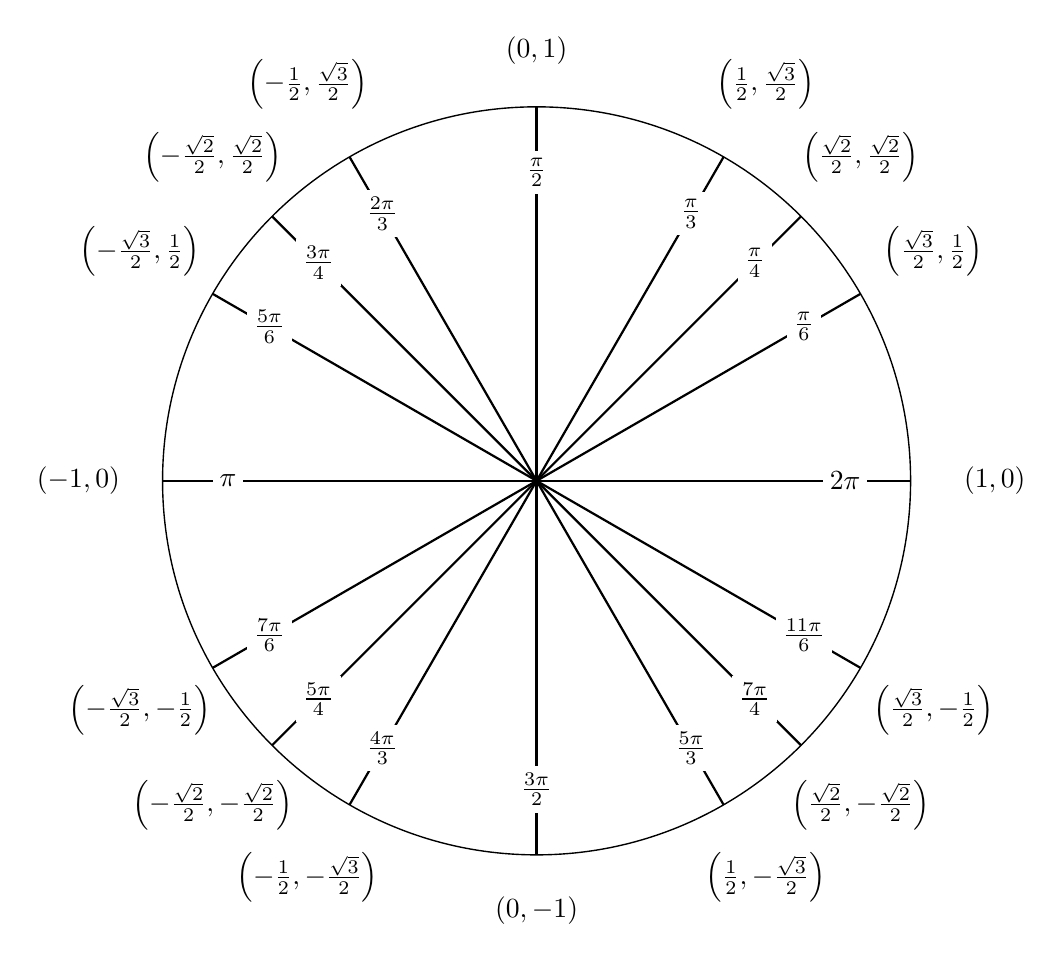
\begin{tikzpicture}[scale=1.0, line width=0.8pt, declare function={
      cRad=4.75; rRad=0.825*cRad; tRad=1.225*cRad;}]
      \draw[line width=0.5pt] (0,0) circle(cRad);
      \foreach \x/\xtext in {
        30/\frac{\pi}{6},    45/\frac{\pi}{4},   60/\frac{\pi}{3},    90/\frac{\pi}{2},
        120/\frac{2\pi}{3}, 135/\frac{3\pi}{4}, 150/\frac{5\pi}{6},  180/\pi,
        210/\frac{7\pi}{6}, 225/\frac{5\pi}{4}, 240/\frac{4\pi}{3},  270/\frac{3\pi}{2},
        300/\frac{5\pi}{3}, 315/\frac{7\pi}{4}, 330/\frac{11\pi}{6}, 360/2\pi}{
          \draw[\lCol] (0cm,0cm) -- (\x:cRad);
          \draw (\x:rRad) node[fill=white, inner sep=2.5pt] {$\xtext$};
        }
    \foreach \x/\xtext/\y in {
      % the coordinates for the first quadrant
      30/\frac{\sqrt{3}}{2}/\frac{1}{2},
      45/\frac{\sqrt{2}}{2}/\frac{\sqrt{2}}{2},
      60/\frac{1}{2}/\frac{\sqrt{3}}{2},
      % the coordinates for the second quadrant
      150/-\frac{\sqrt{3}}{2}/\frac{1}{2},
      135/-\frac{\sqrt{2}}{2}/\frac{\sqrt{2}}{2},
      120/-\frac{1}{2}/\frac{\sqrt{3}}{2},
      % the coordinates for the third quadrant
      210/-\frac{\sqrt{3}}{2}/-\frac{1}{2},
      225/-\frac{\sqrt{2}}{2}/-\frac{\sqrt{2}}{2},
      240/-\frac{1}{2}/-\frac{\sqrt{3}}{2},
      % the coordinates for the fourth quadrant
      330/\frac{\sqrt{3}}{2}/-\frac{1}{2},
      315/\frac{\sqrt{2}}{2}/-\frac{\sqrt{2}}{2},
      300/\frac{1}{2}/-\frac{\sqrt{3}}{2}}
        \draw (\x:tRad) node {$\left(\xtext,\y\right)$};
        \draw (-tRad,0cm) node{$(-1,0)$}
              (tRad,0cm)  node{$(1,0)$}
              (0cm,-cRad*1.15) node{$(0,-1)$}
              (0cm,cRad*1.15)  node{$(0,1)$};
    \end{tikzpicture}
  \end{center}
  \vspace*{\stretch{1}}

  \begin{defn*}[Positive Orientation]
    The direction in which a parametric curve is generated as the parameter increases is called the \textbf{positive orientation} of the curve (and is indicated by arrows on the curve).
  \end{defn*}
  \pagebreak

  \begin{ex*}[\textcolor{blue}{LC 32.1-32.2}]
    Consider the parametric equations
      \[x=3\cos(t),\ y=3\sin(t); \pi\leq t\leq 2\pi\]
  \end{ex*}
  \begin{tasks}[after-item-skip=\stretch{1}, label=,item-indent=0pt](1)
    \task Eliminate the parameter $t$ and rewrite as a function of $x$ and $y$.
    \task Graph the equation found above indicating the positive orientation.
  \end{tasks}
  \begin{center}
    \begin{tikzpicture}[scale=1.1]
      \begin{axis}[
        axis lines=center,
        axis line style={black,->},
        xmin=-4.5, xmax=4.5,
        ymin=-4.5, ymax=4.5,
        xtick={-6,-5,...,6},
        xticklabels={},
        ytick={-6,-5,...,6},
        yticklabels={},
        ticklabel style={font=\footnotesize,inner sep=0.5pt,fill=white,opacity=1.0, text opacity=1},
        xlabel=$x(t)$, xlabel style={at={(ticklabel* cs:1)},anchor=north west},
        ylabel=$y(t)$, ylabel style={at={(ticklabel* cs:1)},anchor=south west},
        every axis plot/.append style={line width=0.95pt, color=blue, samples=100}
        ]
      \end{axis}
    \end{tikzpicture}
  \end{center}
  \pagebreak

  \begin{ex*}[\textcolor{blue}{LC 32.3-32.4}]
    A Ferris wheel has a radius of $20$ m and completes a revolution in the \textbf{clockwise} direction at constant speed in $3$ minutes.  Assume $x$ and $y$ measure the horizontal and vertical positions of a seat on the Ferris wheel relative to a coordinate system whose origin is at the low point of the wheel.  Assume the seat begins moving at the origin.
  \end{ex*}
  \begin{flushright}
    \smash{\raisebox{-\height+1.5\baselineskip}{
    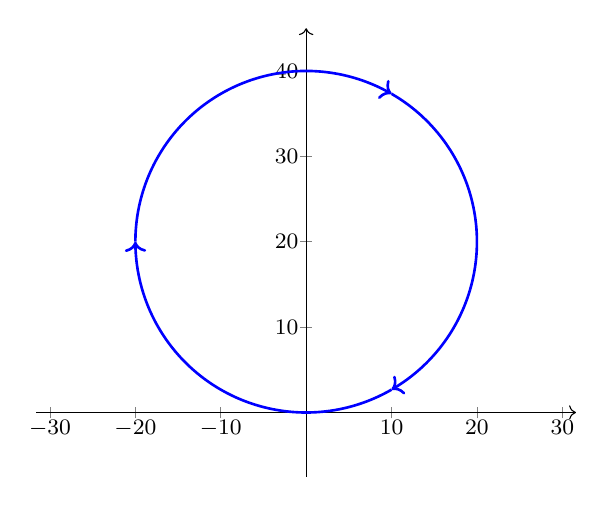
\begin{tikzpicture}[declare function={
      c=0; d=20;}]
      \begin{axis}[
          axis lines=center,
          axis line style={black,->},
          axis equal,
          ymin=-7.5, ymax=45,
          ticklabel style={font=\footnotesize,inner sep=0.5pt,fill=white,opacity=1.0, text opacity=1},
          every axis plot/.append style={line width=0.95pt, color=blue, samples=100}
        ]
        \addplot[<-, data cs=polar, domain=-45:15] (x,{2*c*cos(x)+2*d*sin(x)});
        \addplot[<-, data cs=polar, domain=15:75] (x,{2*c*cos(x)+2*d*sin(x)});
        \addplot[<-, data cs=polar, domain=75:135] (x,{2*c*cos(x)+2*d*sin(x)});
      \end{axis}
    \end{tikzpicture}}}
  \end{flushright}
  \vspace*{-1.5\baselineskip}
  \begin{tasks}[after-item-skip=\stretch{1}, label=,item-indent=0pt](1)
    \task \parbox{0.7\linewidth}{What is the domain of $t$ such that the Ferris wheel completes one revolution?}
    \task $x(t)$ and $y(t)$ will be parameterized using $\sin(bt)$ and $\cos(bt)$. What is $b$?
    \task What parametric equations describe the path of the seat on the Ferris wheel?
  \end{tasks}
  \vspace*{\stretch{1}}
  \pagebreak

  \begin{thmBox*}[Summary: Parametric Equations of a Line]
    The equations
      \[x=x_0+at,\ y=y_0+bt,\ \textnormal{ for } -\infty<t<\infty,\]
    where $x_0$, $y_0$, $a$, and $b$ are constants with $a\neq 0$, describe a line with slope $\frac{b}{a}$ passing through the point $(x_0,y_0)$. If $a=0$ and $b\neq0$, the line is vertical.
  \end{thmBox*}

  \begin{ex*}
    Find 2 parameterized equations of the line that goes through the points $(3,-4)$ and $(-2,3)$.
  \end{ex*}
  \vspace*{\stretch{1}}

  \begin{ex*}
    Find a parameterized equation for the line segment that connects the points $(3,0)$ and $(-1,3)$.
  \end{ex*}
  \vspace*{\stretch{1}}
  \pagebreak

  \begin{ex*}
    Consider the parametric equations 
      \[x(t)=6-2t \textnormal{ and } y(t)=-2+t,\] 
  \end{ex*}
  \begin{tasks}[after-item-skip=\stretch{0}, label=,item-indent=0pt](1)
    \task Graph the curve indicating the positive orientation
      \begin{center}
        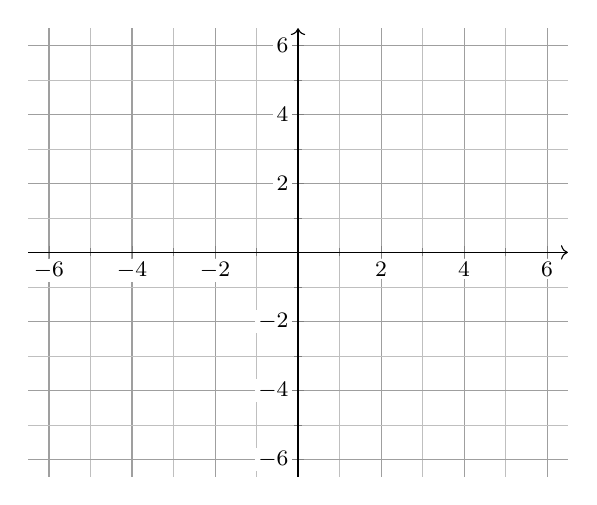
\begin{tikzpicture}[declare function={
          c=0; d=20;}]
          \begin{axis}[
            grid=both, %major,minor
            grid style={line width=0.3pt, draw=gray!60},
            major grid style={line width=0.375pt, draw=gray!75},
            minor grid style={line width=0.15pt, draw=gray!50},
            axis lines=center,
            axis line style={black,->},
            xmin=-6.5, xmax=6.5,
            ymin=-6.5, ymax=6.5,
            minor x tick num=1,
            minor y tick num=1,
            ticklabel style={font=\footnotesize,inner sep=1.15pt,fill=white,opacity=1.0, text opacity=1},
            every axis plot/.append style={line width=0.95pt, color=blue, samples=100}
            ]
          \end{axis}
        \end{tikzpicture}
      \end{center}
    \task Eliminate the parameter to find an equation in $x$ and $y$.
  \end{tasks}
  \vspace*{\stretch{1}}
  \pagebreak

  \begin{ex*}[\textcolor{blue}{LC 32.5-32.7}]
    Consider the parametric equations
      \[x=1+e^{2t}\textnormal{ and } y=e^t,\]
  \end{ex*}
  \begin{tasks}[after-item-skip=\stretch{1}, label=,item-indent=0pt](1)
    \task Eliminate the parameter to find an equation in $x$ and $y$
    \task Graph the curve indicating the positive orientation
      \begin{center}
        \smash{\raisebox{-\height+\baselineskip}{
          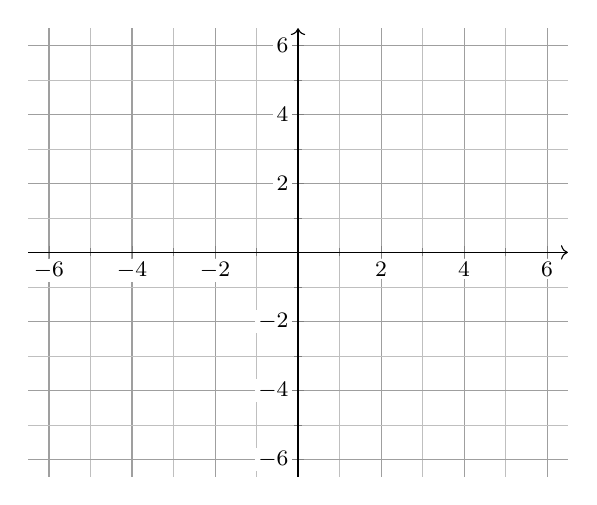
\begin{tikzpicture}[scale=1.0]
            \begin{axis}[
              grid=both, %major,minor
              grid style={line width=0.3pt, draw=gray!60},
              major grid style={line width=0.375pt, draw=gray!75},
              minor grid style={line width=0.15pt, draw=gray!50},
              axis lines=center,
              axis line style={black,->},
              xmin=-6.5, xmax=6.5,
              ymin=-6.5, ymax=6.5,
              minor x tick num=1,
              minor y tick num=1,
              ticklabel style={font=\footnotesize,inner sep=1.15pt,fill=white,opacity=1.0, text opacity=1},
              every axis plot/.append style={line width=0.95pt, color=blue, samples=100}
              ]
            \end{axis}
          \end{tikzpicture}
        }}
      \end{center}
    \task Which of the following parametric equations are equivalent?
    \begingroup
    \addtolength{\jot}{5mm}
    \begin{alignat*}{3}
      x&=2t^2, \hspace*{15mm} &y&=4+t;\hspace*{15mm} &-4\leq{}& t\leq 4\\
      x&=2t^4, &y&=4+t^2; &-2\leq{}& t\leq 2\\
      x&=2t^{2/3}, &y&=4+t^{1/3}; &-64\leq{}& t\leq 64
    \end{alignat*}
    \endgroup
  \end{tasks}
  \pagebreak

  \begin{thmBox*}[Theorem 12.1: Derivative for Parametric Curves]
    Let $x=f(t)$ and $y=g(t)$, where $f$ and $g$ are differentiable on an interval $[a,b]$. Then the slope of the line tangent to the curve at the point corresponding to $t$ is
      \[\frac{dy}{dx}=\frac{dy/dt}{dx/dt}=\frac{g'(t)}{f'(t)},\]
    provided $f'(t)\neq 0$.
  \end{thmBox*}
  \begin{ex*}[\textcolor{blue}{LC 32.8-32.9}]
    Consider the parametric equations
      \[x=\sqrt{t},\qquad y=2t,\]
  \end{ex*}
  \begin{tasks}[after-item-skip=\stretch{1}, label=,item-indent=0pt](1)
    \task Find $\dfrac{dy}{dt}$.
    \task Find the equation of the line tangent to the curve at $t=4$.
  \end{tasks}
  \vspace*{\stretch{1}}
  \pagebreak

  \begin{defn*}[Arc Length for Curves Defined by Parametric Equations]
    Consider the curve described by the parametric equations $x=f(t)$, $y=g(t)$, where $f'$ and $g'$ are continuous, and the curve is traversed once for $a\leq t\leq b$. The \textbf{arc length} of the curve between $\parens{f(a),g(a)}$ and $\parens{f(b),g(b)}$ is
      \[L=\int_a^b \sqrt{f'(t)^2+g'(t)^2}\,dt.\]
  \end{defn*}

  \begin{ex*}[\textcolor{blue}{LC 33.1-33.2}]
    Find the arc length of the curve given by $x=6t^2$, $y=2t^3$, for $0\leq t\leq 4$.
  \end{ex*}
  \vspace*{\stretch{1}}
  \pagebreak

  \begin{ex*}
    Suppose the function $y=h(x)$ is nonnegative and continuous on $[\alpha,\beta]$, which implies that the area bounded by the graph of $h$ and the $x$-axis on $[\alpha,\beta]$ equals $\int_\alpha^\beta h(x)\,dx$ or $\int_\alpha^\beta y\,dx$. If the graph of $y=h(x)$ on $[\alpha,\beta]$ is traced exactly once by the parametric equations $x=f(t)$, $y=g(t)$, for $a\leq t\leq b$, then it follows by substitution that the area bounded by $h$ is
      \[\int_\alpha^\beta h(x)\,dx=\int_a^b g(t)f'(t)\,dt \textnormal{ if }\alpha=f(a) \textnormal{ and } \beta=f(b)\]
    Find the area under one arch of the cycloid $x=3(t-\sin(t))$, $y=3(1-\cos(t))$.
  \end{ex*}
  \begin{center}
    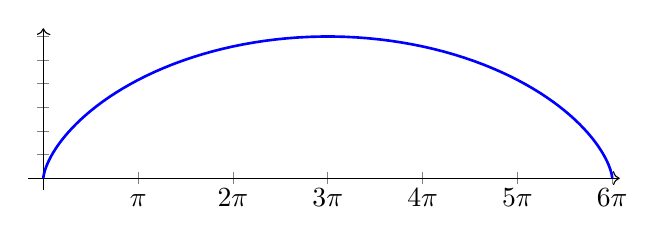
\begin{tikzpicture}
      \begin{axis}[
        axis lines=center,
        axis line style={black,->},
        xmin=-0.5, xmax=6*pi+0.25,
        ymin=-0.5, ymax=6.35,
        xtick={0,pi,2*pi,3*pi,4*pi,5*pi,6*pi},
        xticklabels={$0$,$\vphantom{2}\pi$,$2\pi$,$3\pi$,$4\pi$,$5\pi$,$6\pi$},
        ytick={-6,-5,...,6},
        yticklabels={},
        ticklabel style={font=\normalsize,inner sep=1.5pt,fill=white,opacity=1.0, text opacity=1},
        every axis plot/.append style={line width=0.95pt, color=blue, samples=100},
        width=0.75\linewidth, height=0.3\linewidth
        ]
        \addplot[-, domain=0:2*pi] ({3*(x-sin(deg(x))},{3*(1-cos(deg(x))});
      \end{axis}
    \end{tikzpicture}
  \end{center}
  \vspace*{\stretch{1}}
  \pagebreak
  
  \begin{ex*}[\textcolor{blue}{33.3} Surface area]
    Let $C$ be the curve $x=f(t)$, $y=g(t)$, for $a\leq t\leq b$, where $f'$ and $g'$ are continuous on $[a,b]$ and $C$ does not intersect itself, except possibly at its endpoints. If $g$ is nonnegative on $[a,b]$, then the area of the surface obtained by revolving $C$ about the $x$-axis is
      \[S=\int_a^b 2\pi g(t)\sqrt{f'(t)^2+g'(t)^2}\,dt.\]
    Setup the integral used to find the area of the surface obtained by revolving the curve $x=t\sin(t)$, $y=t\cos(t)$, for $0\leq t\leq \pi/2$, about the $x$-axis.
  \end{ex*}
  \vspace*{\stretch{1}}
  \pagebreak

\end{document}

%  \documentclass[../mathNotesPreamble]{subfiles}
\begin{document}
\relscale{1.4}
  \section{12.2: Polar Coordinates}

  \noindent\textbf{Defining Polar Coordinates}
    When using polar coordinates, the origin of the coordinate system is called the \textbf{pole}, and the positive $x$-axis is called the \textbf{polar axis}. The polar coordinates for a point $P$ are of the form $(r,\theta)$. \newline 
    The \textbf{radial coordinate} $r$ describes the \textit{signed} (\textit{directed}) distance from the origin to $P$.\newline 
    The \textbf{angular coordinate} $\theta$ describes an angle whose initial side is the positive $x$-axis and whose terminal side lies on the ray passing through the origin and $P$.

  \begin{ex*}[\textcolor{blue}{LC 33.4}]
    Graph the following polar coordinates
  \end{ex*}
  \begin{tasks}[after-item-skip=\stretch{0}, label=\Alph*)](4)
    \task $\parens{\dfrac{3}{2},\dfrac{\pi}{2}}$
    \task $\parens{1,\dfrac{5\pi}{3}}$
    \task $\parens{\dfrac{3}{2},\dfrac{7\pi}{4}}$
    \task $\parens{-1,\dfrac{-\pi}{3}}$
  \end{tasks}
  \vspace*{\stretch{1}}
  \begin{center}
    \begin{tikzpicture}[scale=1.4]
      \begin{polaraxis}
        [
        axis on top,
        domain=0:360,
        samples=180,
        grid=both,
        grid style={line width=0.1pt, draw=gray!75},
        major grid style={black, line width=0.5pt},
        minor grid style={black!60, line width=0.15pt}, 
        minor x tick num=1,
        minor y tick num=1,
        xmin=0, xmax=360,
        ymin=0, ymax=1.5,
        xtick={0,30,...,360},
        xticklabels={$0$,,,$\frac{\pi}{2}$,,,$\pi$,,,$\frac{3\pi}{2}$,,,},
        ytick={0,1},
        yticklabels={,$1$},
        yticklabel style={anchor=north west, inner sep=1.0pt, fill=white, opacity=0.5, text opacity=1.0, font=\normalsize},
        every axis plot/.append style={line width=0.5pt, color=blue, samples=360}
        ]
      \end{polaraxis}
    \end{tikzpicture}
  \end{center}
  \vspace*{\stretch{1}}
  \pagebreak

  \begin{thmBox*}[Procedure: Converting Coordinates]
    A point with polar coordinates $(r,\theta)$ has Cartesian coordinates $(x,y)$, where
      \[x=r\cos\theta \qquad\textnormal{ and }\qquad y=r\sin\theta.\]
    A point with Cartesian coordinates $(x,y)$ has polar coordinates $(r,\theta)$, where 
      \[r^2=x^2+y^2 \qquad \textnormal{ and }\qquad \tan\theta=\frac{y}{x}.\]
  \end{thmBox*}

  \begin{ex*}[\textcolor{blue}{LC 33.5}]
    Consider the Cartesian coordinate $\parens{4\sqrt{3},-4}$. Rewrite this point in polar coordinates. \hspace*{\stretch{1}} \textit{Note}: There are infinitely many polar representations
  \end{ex*}
  \vspace*{\stretch{1}}

  \begin{ex*}[\textcolor{blue}{LC 33.6}]
    Rewrite $y=3$ in terms of polar coordinates.
  \end{ex*}
  \vspace*{\stretch{1}}

  \begin{ex*}[\textcolor{blue}{LC 33.7}]
    Graph $r=4$ and $\theta=\frac{2\pi}{3}$
  \end{ex*}
  \vspace*{\stretch{1}}
  \begin{flushright}
    \smash{
    \begin{tikzpicture}
      \begin{polaraxis}[
        axis on top,
        domain=0:360,
        samples=180,
        grid=both,
        grid style={line width=0.1pt, draw=gray!75},
        major grid style={black, line width=0.5pt},
        minor grid style={black!60, line width=0.15pt}, 
        xmin=0, xmax=360,
        ymin=0, ymax=5,
        xtick={0,30,...,360},
        xticklabels={},
        yticklabels={,,$2$,$4$},
        yticklabel style={anchor=north west, inner sep=1.0pt, fill=white, opacity=0.5, text opacity=1.0, font=\normalsize},
        every axis plot/.append style={line width=0.5pt, color=blue, samples=360}
        ]
      \end{polaraxis}
    \end{tikzpicture}}
  \end{flushright}
  \pagebreak

  \begin{thmBox*}[Summary: Circles in Polar Coordinates]
    The equation $r=a$ describes a circle of radius $\abs{a}$ centered at $(0,0)$.\newline
    The equation $r=2a\cos\theta+2b\sin\theta$ describes a circle of radius $\sqrt{a^2+b^2}$ centered at $(a,b)$.
    \begin{center}
      \begin{tikzpicture}[declare function={
        a=2; b=1.5; 
        aa=a/sqrt(a^2+b^2); bb=b/sqrt(a^2+b^2);}]
        \begin{axis}[
          axis lines=center,
          axis line style={black,->},
          axis equal,
          xmin=-1.35, xmax=1.35,
          ymin=-1.35, ymax=1.35,
          xmajorticks=false,
          ymajorticks=false,
          ticklabel style={font=\footnotesize,inner sep=0.5pt,fill=white,opacity=1.0, text opacity=1},
          xlabel=$x$, xlabel style={at={(ticklabel* cs:1)},anchor=north west},
          ylabel=$y$, ylabel style={at={(ticklabel* cs:1)},anchor=south west},
          every axis plot/.append style={line width=0.95pt, color=blue, samples=100}
          ]
            \addplot[data cs=polar, domain=0:360] (x,{1}) node[above right, black, pos=0.175, font=\normalsize] {$r=a$};
            \addplot[soldot, red] coordinates{(0,0)} node[below left, black, font=\normalsize] {$(0,0)$};
            \draw[red] (axis cs: 0,0) -- (axis cs: aa,bb) node[above, pos=0.45, font=\normalsize] {$\abs{a}$};
        \end{axis}
      \end{tikzpicture}
      \hspace*{15mm}
      \begin{tikzpicture}[declare function={
        a=2; b=1; 
        aa=a/sqrt(a^2+b^2); bb=b/sqrt(a^2+b^2);
        c=3/5; d=4/5;}]
        \begin{axis}[
          axis lines=center,
          axis line style={black,->},
          axis equal,
          xmin=-0.5, xmax=2.15,
          ymin=-0.5, ymax=2.25,
          xmajorticks=false,
          ymajorticks=false,
          ticklabel style={font=\footnotesize,inner sep=0.5pt,fill=white,opacity=1.0, text opacity=1},
          xlabel=$x$, xlabel style={at={(ticklabel* cs:1)},anchor=north west},
          ylabel=$y$, ylabel style={at={(ticklabel* cs:1)},anchor=south west},
          every axis plot/.append style={line width=0.95pt, color=blue, samples=100}
          ]
            \addplot[data cs=polar, domain=0:360] (x,{2*c*cos(x)+2*d*sin(x)}) node[above, black, pos=0.15, yshift=10pt, font=\normalsize] {$r=2a\cos(\theta)+2b\sin(\theta)$};
            \addplot[soldot, red] coordinates{(0,0)} node[below left, black, font=\normalsize] {$O$};
            \addplot[soldot, black] coordinates{(c,d)} node[above, black, font=\normalsize] {$(a,b)$};
            \draw[red] (axis cs: 0,0) -- (axis cs: c,d) node[right, pos=0.45, font=\normalsize] {$\sqrt{a^2+b^2}$};
        \end{axis}
      \end{tikzpicture}
    \end{center}
  \end{thmBox*}

  \begin{ex*}
    Rewrite the following in either polar coordinates or Cartesian coordinates
  \end{ex*}
  \begin{tasks}[after-item-skip=\stretch{1}, label=,item-indent=0pt](2)
    \task $r=\cos\theta+2\sin\theta$
    \task $ $
    \task 
    \task 
  \end{tasks}
  \vspace*{\stretch{1}}
  \pagebreak

  \begin{thmBox*}[Procedure: Cartesian-to-Polar Method for Graphing $r=f(\theta)$]
    \begin{enumerate}
      \item Graph $r=f(\theta)$ as if $r$ and $\theta$ were Caresian coordinates with $\theta$ on the horizontal axis and $r$ on the vertical axis. Be sure to choose an interval for $\theta$ on which the entire polar curve is produced.
      \item Use the Cartesian graph that you created in Step 1 as a guide to sketch the points $(r,\theta)$ on the final \textit{polar} curve.
    \end{enumerate}
  \end{thmBox*}

  \begin{thmBox*}[Summary: Symmetry in Polar Equations]
    \begin{description}
      \item[Symmetry about the $x$-axis] occurs if the point $(r,\theta)$ is on the graph whenever $(r,-\theta)$ is on the graph.
      \item[Symmetry about the $y$-axis] occurs if the point $(r,\theta)$ is on the graph whenever $r,\pi-\theta)=(-r,-\theta)$ is on the graph.
      \item[Symmetry about the origin] occurs if the point $(r,\theta)$ is on the graph whenever $(-r,\theta)=(r,\theta+\pi)$ is on the graph.
    \end{description}
  \end{thmBox*}

\end{document}

%  \documentclass[../mathNotesPreamble]{subfiles}
\begin{document}
\relscale{1.4}
  \section{12.3: Calculus in Polar Coordinates}

  \begin{thmBox*}[Theorem 12.2: Slope of a Tangent Line]
    Let $f$ be a differentiable function at $\theta_0$. The slope of the line tangent to the curve $r=f(\theta)$ at the point $(f(\theta_0),\theta_0)$ is
      \[\frac{dy}{dx}=\frac{f'(\theta_0)\sin(\theta_0)+f(\theta_0)\cos(\theta_0)}{f'(\theta_0)\cos(\theta_0)-f(\theta_0)\sin(\theta_0)},\]
    provided the denominator is nonzero at the point. At angles $\theta_0$ for which $f(\theta_0)=0$, $f'(\theta_0)\neq0$, and $\cos(\theta_0)\neq 0$, the tangent line is $\theta=\theta_0$ with slope $\tan(\theta_0)$.
  \end{thmBox*}

  \begin{defn*}[Area of Regions in Polar Coordinates]
    Let $R$ be the region bounded by the graphs of $r=f(\theta)$ and $r=g(\theta)$, between $\theta=\alpha$ and $\theta=\beta$, where $f$ and $g$ are continuous and $f(\theta)\geq g(\theta)\geq 0$ on $[\alpha,\beta]$. The area of $R$ is
      \[\int_\alpha^\beta \frac{1}{2}\parens{f(\theta)^2-g(\theta)^2}\,d\theta.\]
  \end{defn*}

  \begin{thmBox*}[Arc Length of a Polar Curve]
    Let $f$ have a continuous derivative on the interval $[\alpha,\beta]$. The \textbf{arc length} of the polar curve $r=f(\theta)$ on $[\alpha,\beta]$ is
      \[L=\int_\alpha^\beta \sqrt{f(\theta)^2+f'(\theta)^2}\,d\theta.\]
  \end{thmBox*}
\end{document}

\end{document}
